\documentclass{article}
\usepackage{import}
\usepackage[utf8]{inputenc}
\usepackage{amsmath}
\usepackage{amssymb}
\usepackage{mathtools}
\usepackage{graphicx}
\usepackage{tabularx}
\usepackage{float}
\usepackage{subfig}
\usepackage{lscape} 
\usepackage{hyperref}
\usepackage{setspace}
\usepackage{booktabs}
\usepackage[authoryear]{natbib}
\usepackage{lmodern}
\usepackage[T1]{fontenc}
\usepackage[bottom]{footmisc}
\newcommand{\indep}{\perp \!\!\! \perp}
\usepackage[nolist]{acronym}
\newcommand\headercell[1]{%
   \smash[b]{\begin{tabular}[t]{@{}c@{}} #1 \end{tabular}}}
\usepackage[a4paper,top=3cm,bottom=2cm,left=3cm,right=3cm,marginparwidth=1.75cm]{geometry}
\usepackage{xcolor}%
\definecolor{webbrown}{rgb}{.6,0,0}
\usepackage{hyperref}%
\hypersetup{%
  breaklinks = true,%
  colorlinks = true,%
  anchorcolor = webbrown,%
  citecolor = webbrown,%
  filecolor = webbrown,%
  linkcolor = webbrown,%
  menucolor = webbrown,%
  urlcolor= webbrown,%
  citebordercolor= 1 0 0,%
  menubordercolor=1 0 0,%
  urlbordercolor=1 0 0,%
  runbordercolor=1 0 0,}
\usepackage{cleveref}

\usepackage{setspace}
\usepackage{enumitem}
\setstretch{1.5} %% set line spacing

\begin{acronym}
  \acro{CI}{confidence interval}
  \acro{RCT}{randomized controlled trial}
  \acro{IV}{instrumental variable}
  \acro{LATE}{local average treatment effect}
  \acro{ATE}{average treatment effect}
  \acro{OLS}{ordinary least squares}
  \acro{RD}{regression discontinuity}
  \acro{MTE}{marginal treatment effect}
  \acro{ATT}{average treatment effect on the treated}
\end{acronym}

\graphicspath{ {../../output/figures/} }

% Wrap table notes
\usepackage{booktabs}
\newcommand{\tabnotes}[2]{\bottomrule \multicolumn{#1}{@{}p{0.70\linewidth}@{}}{\footnotesize #2 }\end{tabular}\end{table}}

\floatplacement{figure}{H}
\floatplacement{table}{H}

\usepackage[toc,page]{appendix}


\title{College Enrollment and Earnings:
\texorpdfstring{\\}{} Examining the Impact of Two Federal Drug Acts}
\author{Ray Huang\thanks{Contact:
    \href{mailto:ray_huang@brown.edu}{ray\_huang@brown.edu}.
     I thank Peter Hull at Brown University for serving as my advisor and for providing me with fantastic feedback. I would also like to thank Alison Lodermeier and Francesco Ferlenga for their guidance and support.}
     \\Brown University, Honors Thesis}

\date{\today}

\begin{document}

\maketitle

\begin{abstract}
\noindent (to be updated abstract) I examine the impact of two federal drug acts on college enrollments and earnings among black males by using a variety of counterfactual groups. The Anti-Drug Act of 1986 transformed the formerly rehabilitation-focused justice system into a punitive one, imposed sentencing minimums and disparities. The Fair Sentencing Act of 2010 undid many of these policies. I construct estimates of the impact of these two acts on black males aged 18-24 using three unique counterfactual groups: 1) white males, 2) black females, and 3) black men aged 28-34. I also leverage the variation between high and low drug arrest states. I estimate that the Anti-Drug Act of 1986 resulted in a change in college enrollment rates between XX and XX and a change in earnings between XX and XX. For this subpopulation, this implies estimates of economic returns to education ranging from XX to XX.

\end{abstract}

\clearpage

\section*{Introduction}

Anti-Drug Act of 1986:
\begin{itemize}[itemsep=0.05mm, parsep=0pt]
  \item Created minimum sentencing laws re possession of many drugs. 
  \item Crack/powdered cocaine was particularly relevant (significantly harder rules on crack, which was cheaper and used by minorities much more, 100-1 ratio)
  \item The law led to an increase in the average time imprisoned for drug crimes from 22 months to 33 months (Shewan)
\end{itemize}


Fair Sentencing Act of 2010:
\begin{itemize}[itemsep=0.05mm, parsep=0pt]
  \item Reduced the disparity between the amount of crack cocaine and powder cocaine needed to trigger certain federal criminal penalties from a 100:1 weight ratio to an 18:1 weight ratio 
  \item Elimated minimum sentencing for crack cocaine 
  \item Congressional Budget Office has estimated that implementing the Fair Sentencing Act of 2010 will reduce the prison population by 1,550 person-years over the time period from 2011–2015, creating a monetary savings of \$42 million during that period 
\end{itemize}

Existing literature:
\begin{itemize}[itemsep=0.05mm, parsep=0pt]
  \item The Labor Market Consequences of Incarceration- Western, Kling, Weiman (2016)
  \item Juvenile Incarceration, Human Capital, and Future Crime: Evidence from Randomly Assigned Judges - Aizer, Doyle (2015)
  \item Evan Rose papers: The Impact of Incarceration on Employment and Earnings, etc
\end{itemize}


\section*{Data}

\begin{itemize}[itemsep=0.05mm, parsep=0pt]
  \item CPS October supplement
  \begin{itemize}
    \item Dropped observations with missing family income data
    \item Edtype is the variable used for college enrollment, 
  \end{itemize}
  \item UCR from ICPSR (missing data problem, many counties failed to report arrest rates for the relevant crimes)
  \begin{itemize}
    \item Arrest data normalized per 100000. State population data are based on U.S. Census Bureau midyear population estimates.
  \end{itemize}
  \item ACS
\end{itemize}

\section*{Empirical/Econometric Methods, Hypotheses tested}

\textbf{Counterfactual groups}
\begin{itemize}[itemsep=0.05mm, parsep=0pt]
  \item Black males vs white males
  \begin{itemize}
    \item Identifying assumption: absent of the Anti-Drug Abuse Act of 1986, black and white male educational outcomes would have trended similarly.
  \end{itemize}
  \item Black males vs black females
  \item Black males aged 18-24 vs black males aged 28-34 at the time of the act
  \item High vs low drug use
\end{itemize}

\textbf{Basic event study model}
\begin{equation} \label{eq:1}
  y_{it} = \alpha_i + \gamma_t + q'_{it} \phi + \sum_{m=-G}^{M} \beta_m z_{i,t-m} + C_{it} +\epsilon_{it}
\end{equation}

where $\alpha_i$ and $\gamma_t$ are individual and time fixed effects, 

\textbf{Empirical tools:}
\begin{itemize}[itemsep=0.05mm, parsep=0pt]
  \item DiD / DDD / Event study.
  \item \begin{itemize}
    \item Using Roth's pretrend \& honest did suggestions
  \end{itemize}
  \item DDIV
\end{itemize}

%%%%%%%%%%%%%%%%%%%%%%%%BIB%%%%%%%%%%%%%%%%%%%%%%%%%%%

\clearpage
\nocite{*}
\singlespacing
\bibliographystyle{jpe}
\bibliography{citations.bib}

%%%%%%%%%%%%%%%%%%%%%%%%FIGURES%%%%%%%%%%%%%%%%%%%%%%%%%%%

\clearpage

   % Arrest rate pre-trends

   \begin{figure}[h]
    \centering
    \caption{Adult Black Arrest Rate Per 100,000}%
    \subfloat[\centering 1986]{{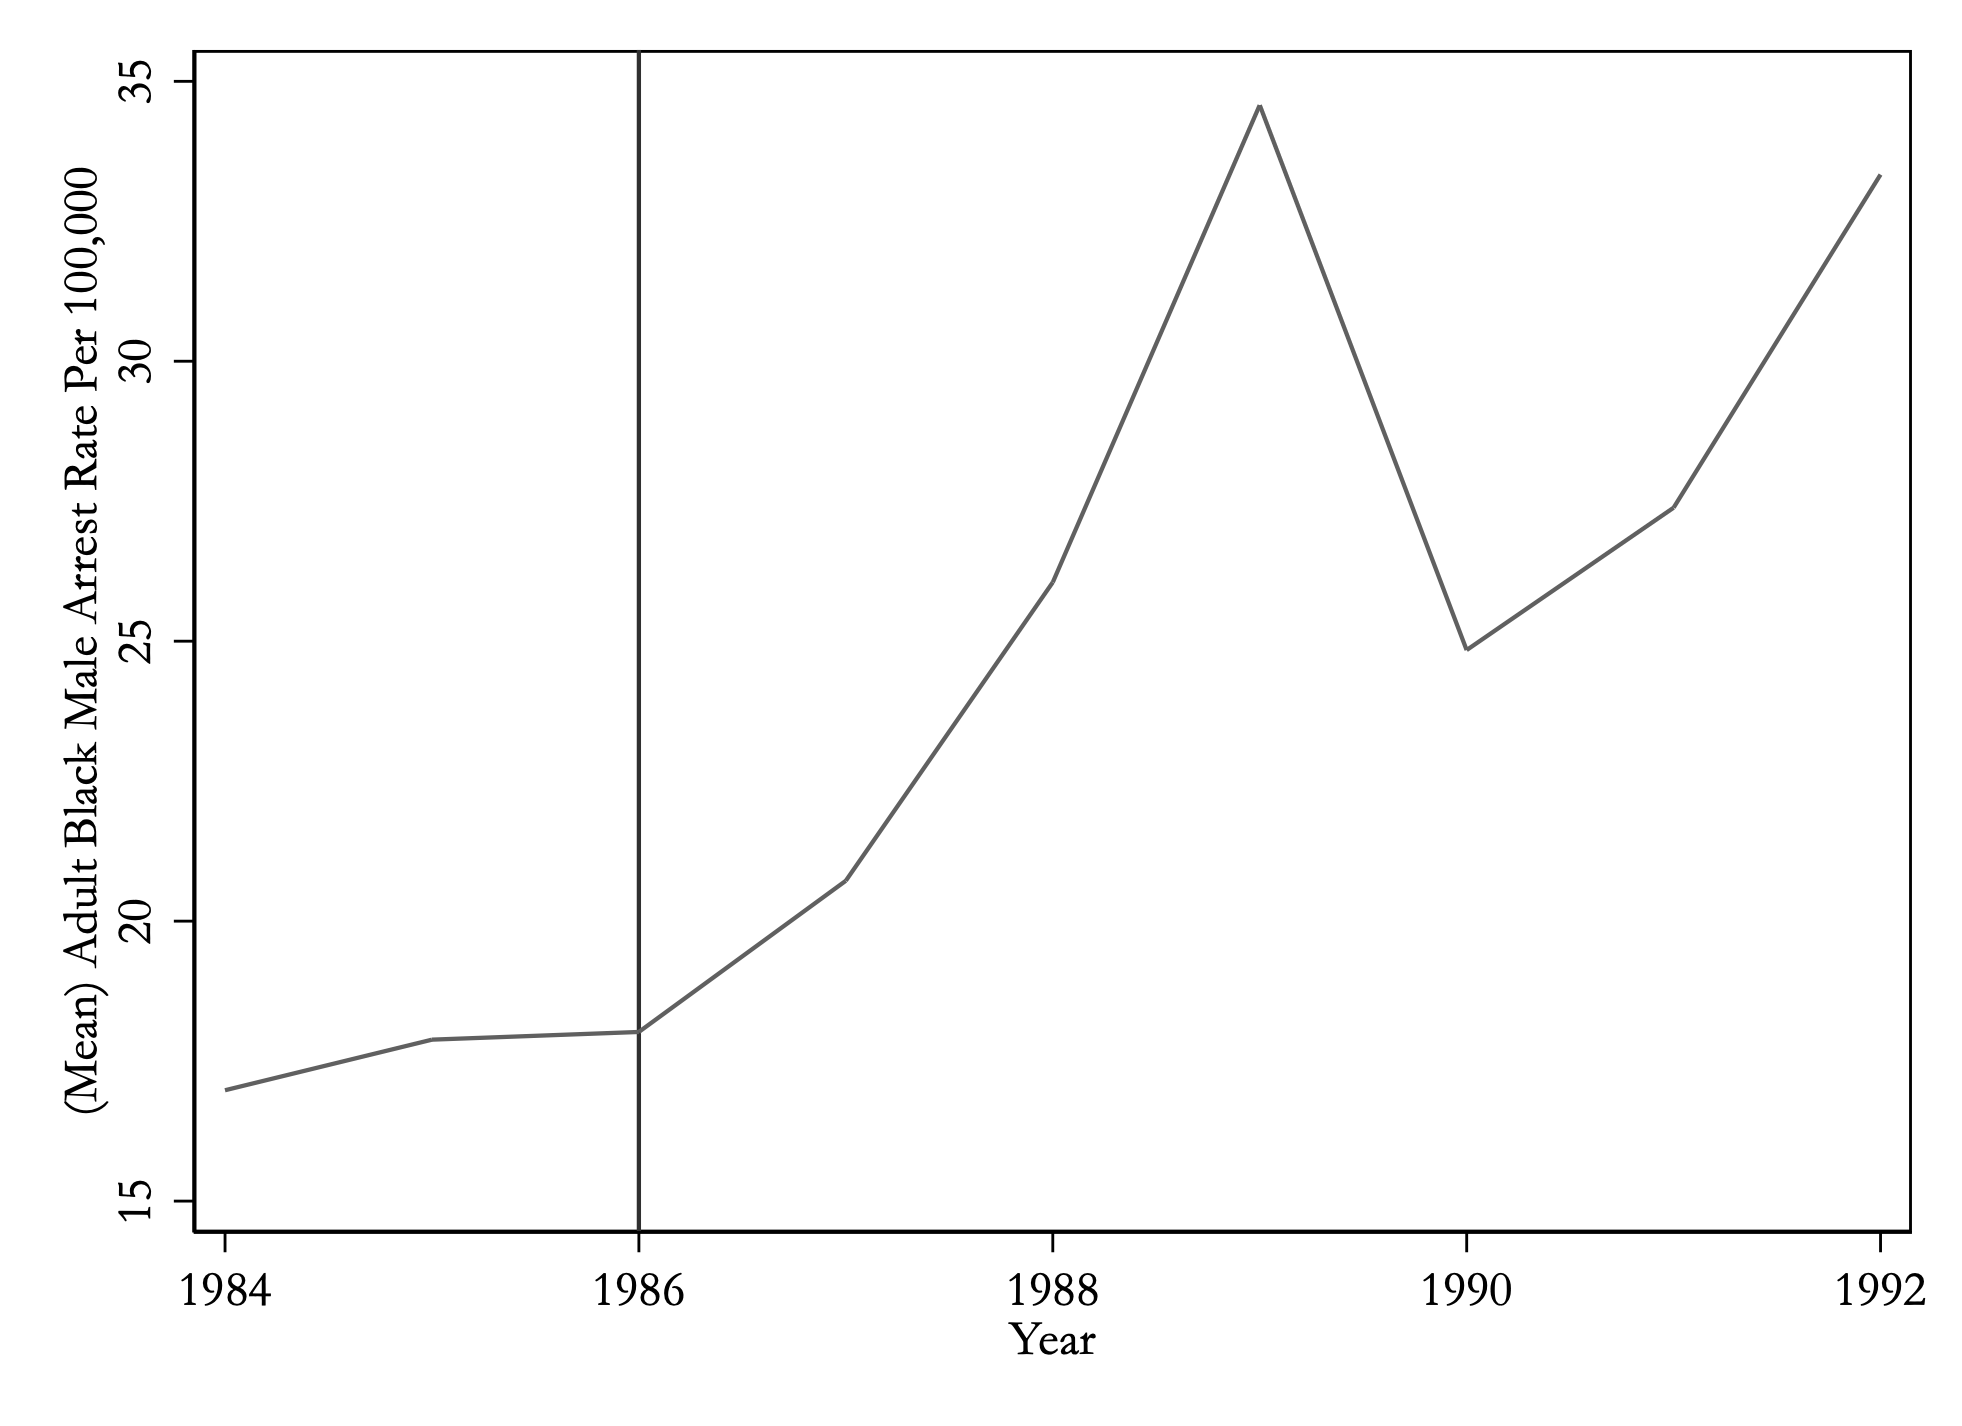
\includegraphics[width=7cm]{pretrends/1986/ab.png} }}%
    \qquad
    \subfloat[\centering 2010]{{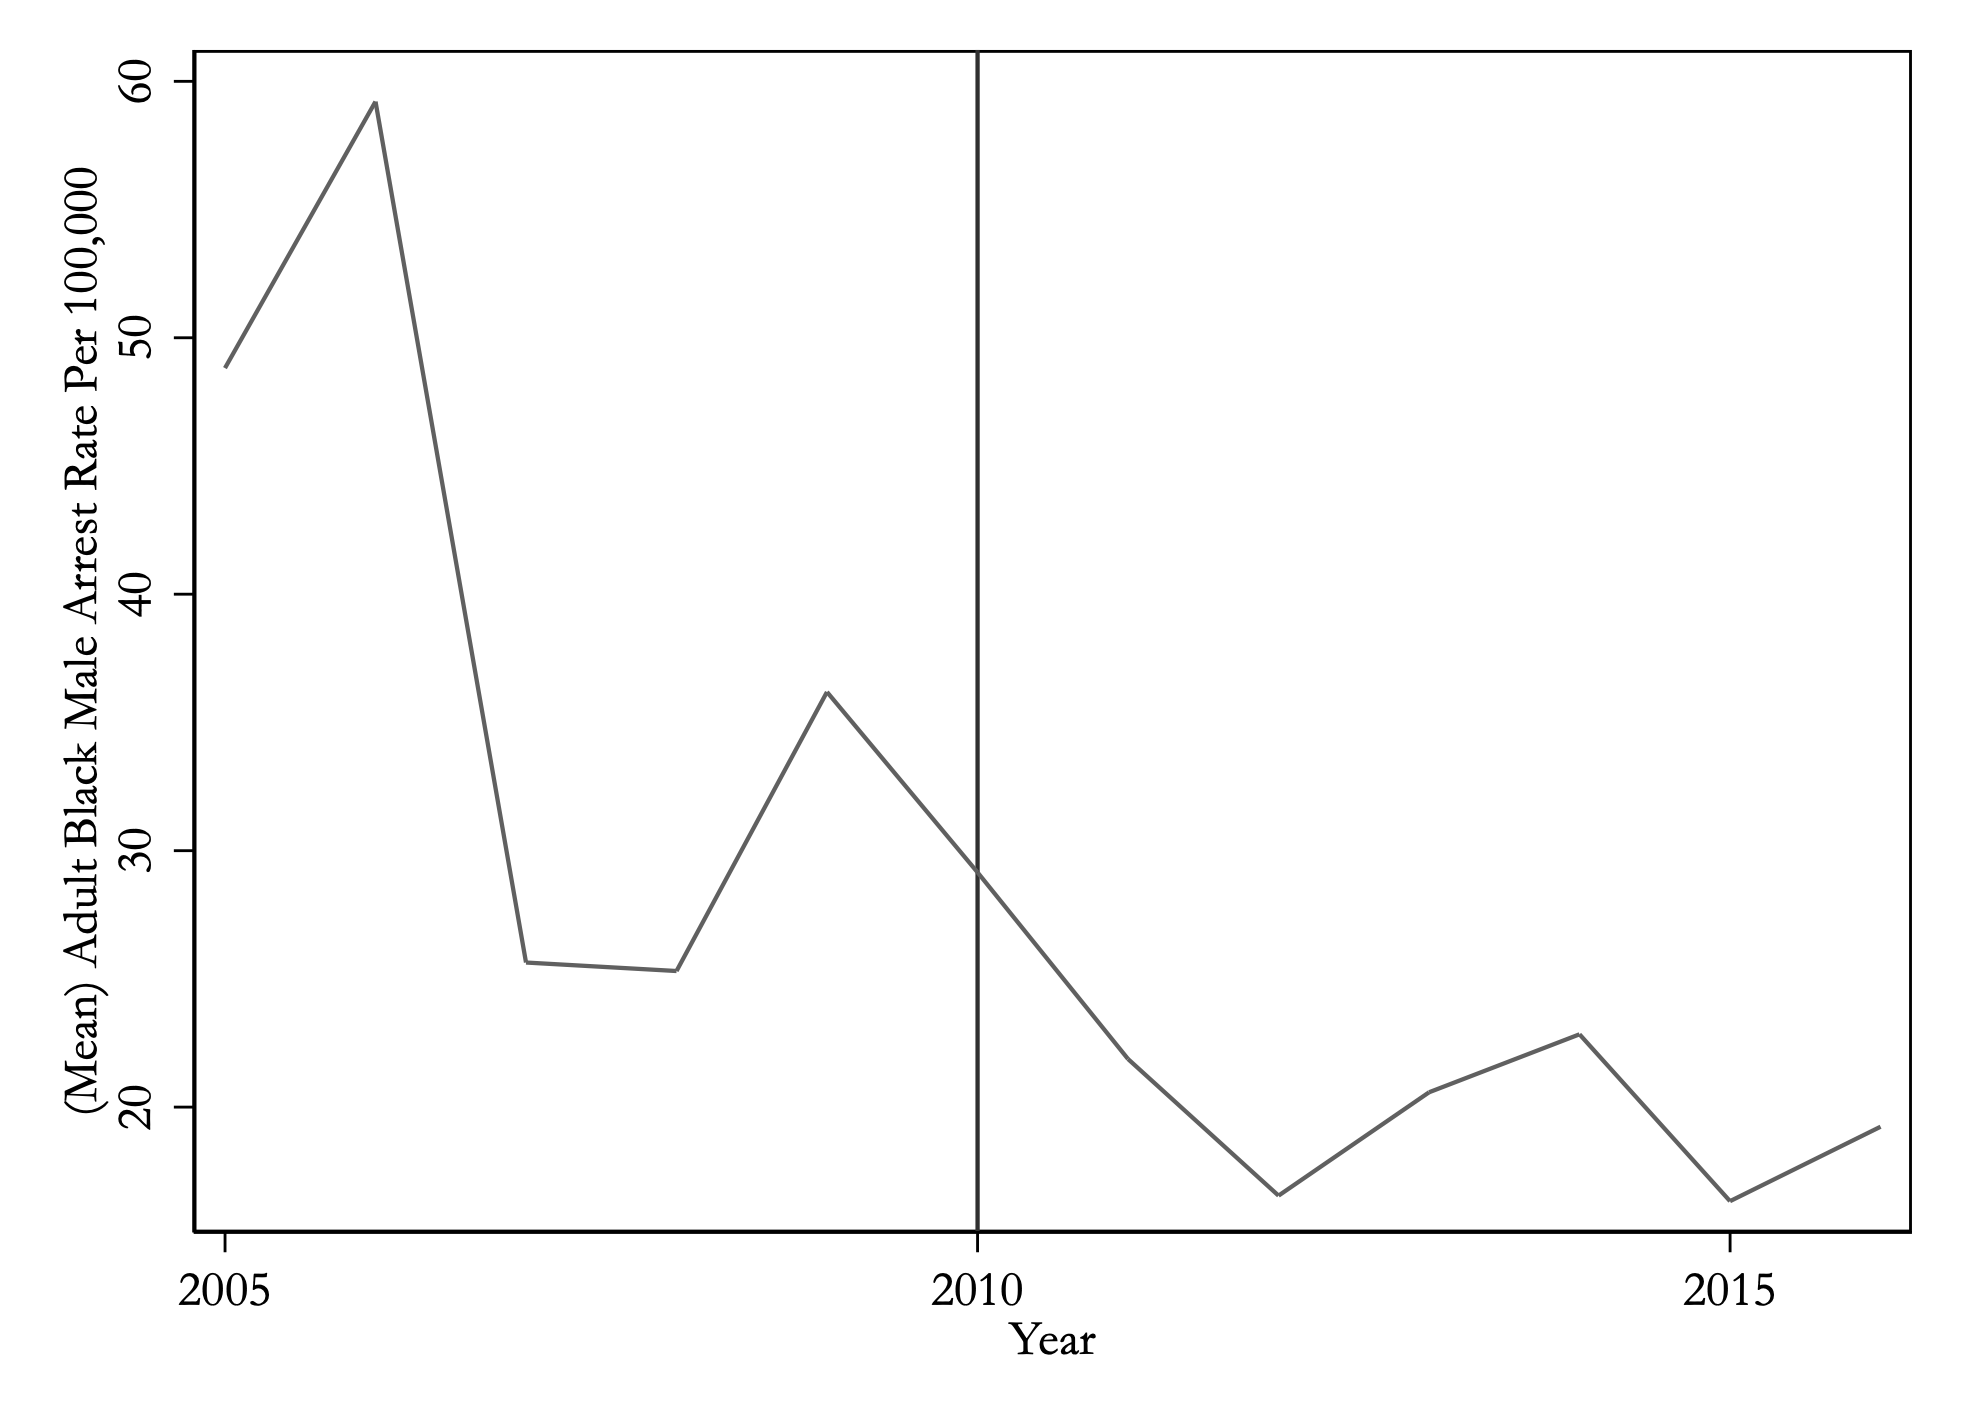
\includegraphics[width=7cm]{pretrends/2010/ab.png} }}%
    \label{fig:raw_ab}%
  \end{figure}
  \begin{figure}[h]
    \centering
    \caption{Juvenile Black Arrest Rate Per 100,000}%
    \subfloat[\centering 1986]{{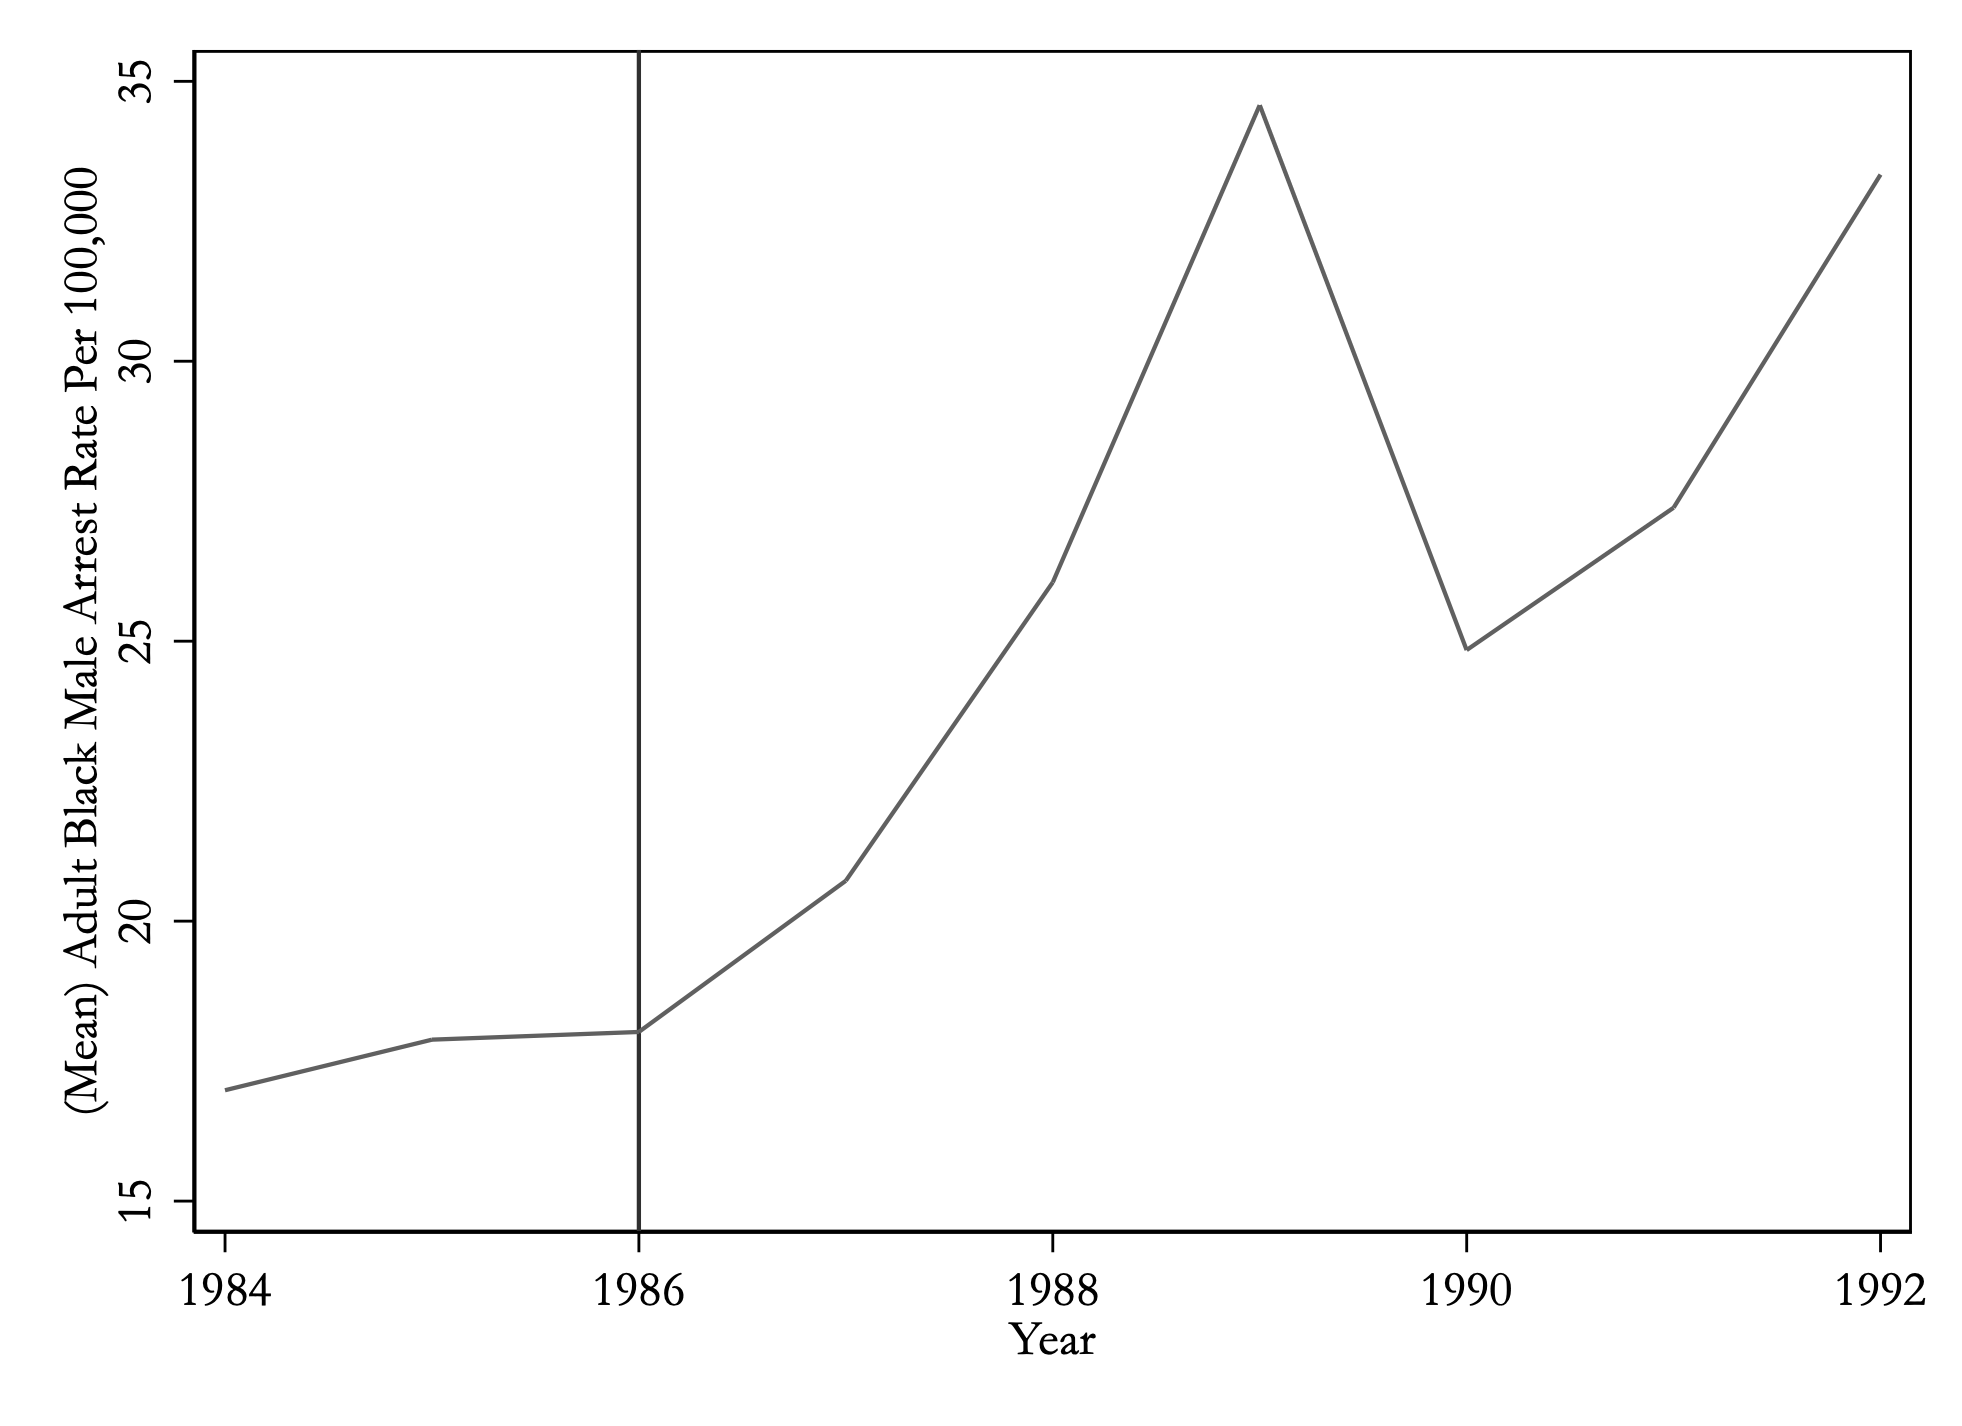
\includegraphics[width=7cm]{pretrends/1986/ab.png} }}%
    \qquad
    \subfloat[\centering 2010]{{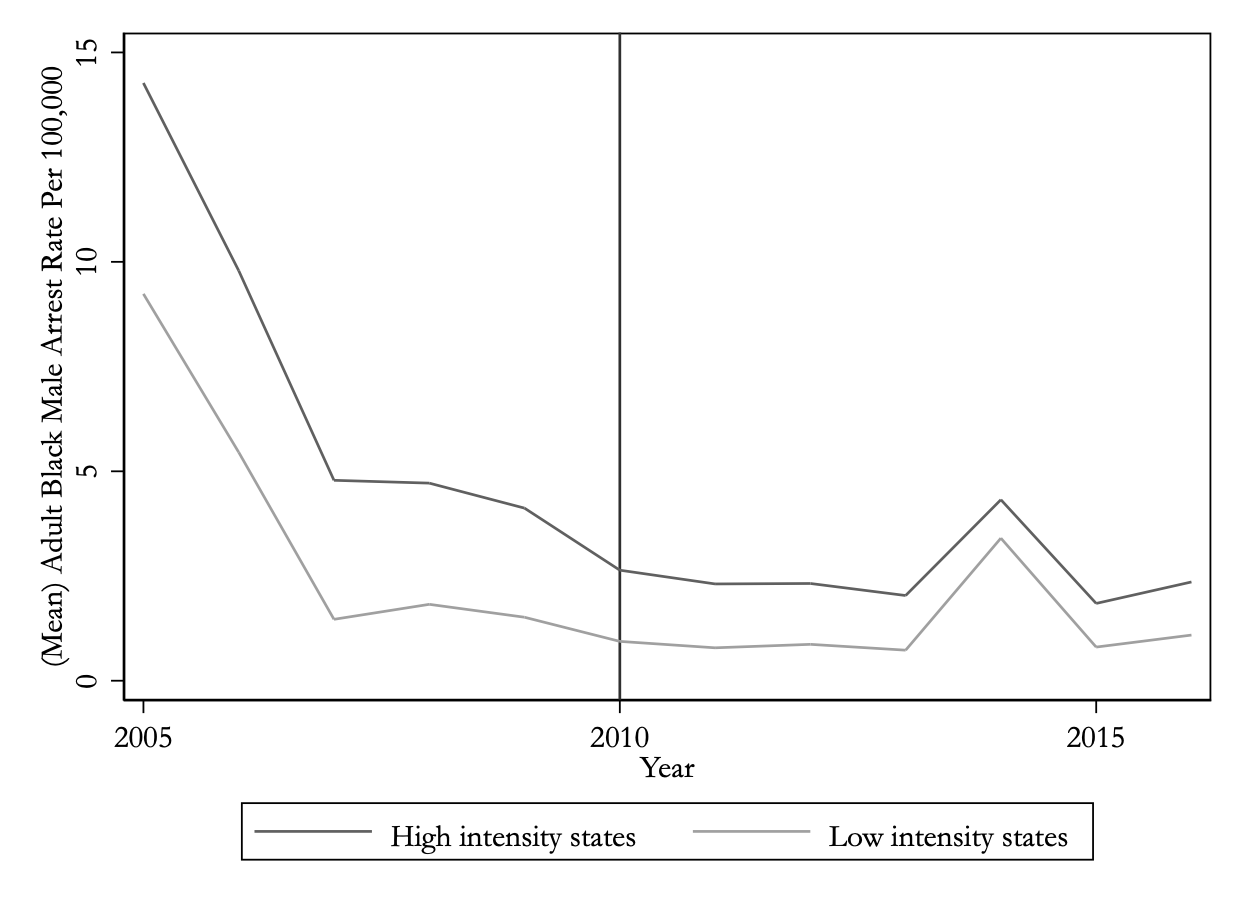
\includegraphics[width=7cm]{pretrends/2010/jb.png} }}%
    \label{fig:raw_jb}%
  \end{figure}

  \begin{footnotesize}
    \noindent Note: These figures report the drug crime arrest rate per 100,000 for black adults and black juveniles separately over time using CPS-UCR merged data from 1984-1992 and 2005-2016. A vertical line is drawn to denote the passage of the Anti-Drug Abuse Act of 1986 and the Fair Sentencing Act of 2010.
  \end{footnotesize}
  
  \clearpage
  
  % High vs low arrest states pre-trends

  \begin{figure}[h]
    \centering
    \caption{College Enrollment By States with High vs Low Black Adult Drug Arrest Rates}%
    \subfloat[\centering 1986]{{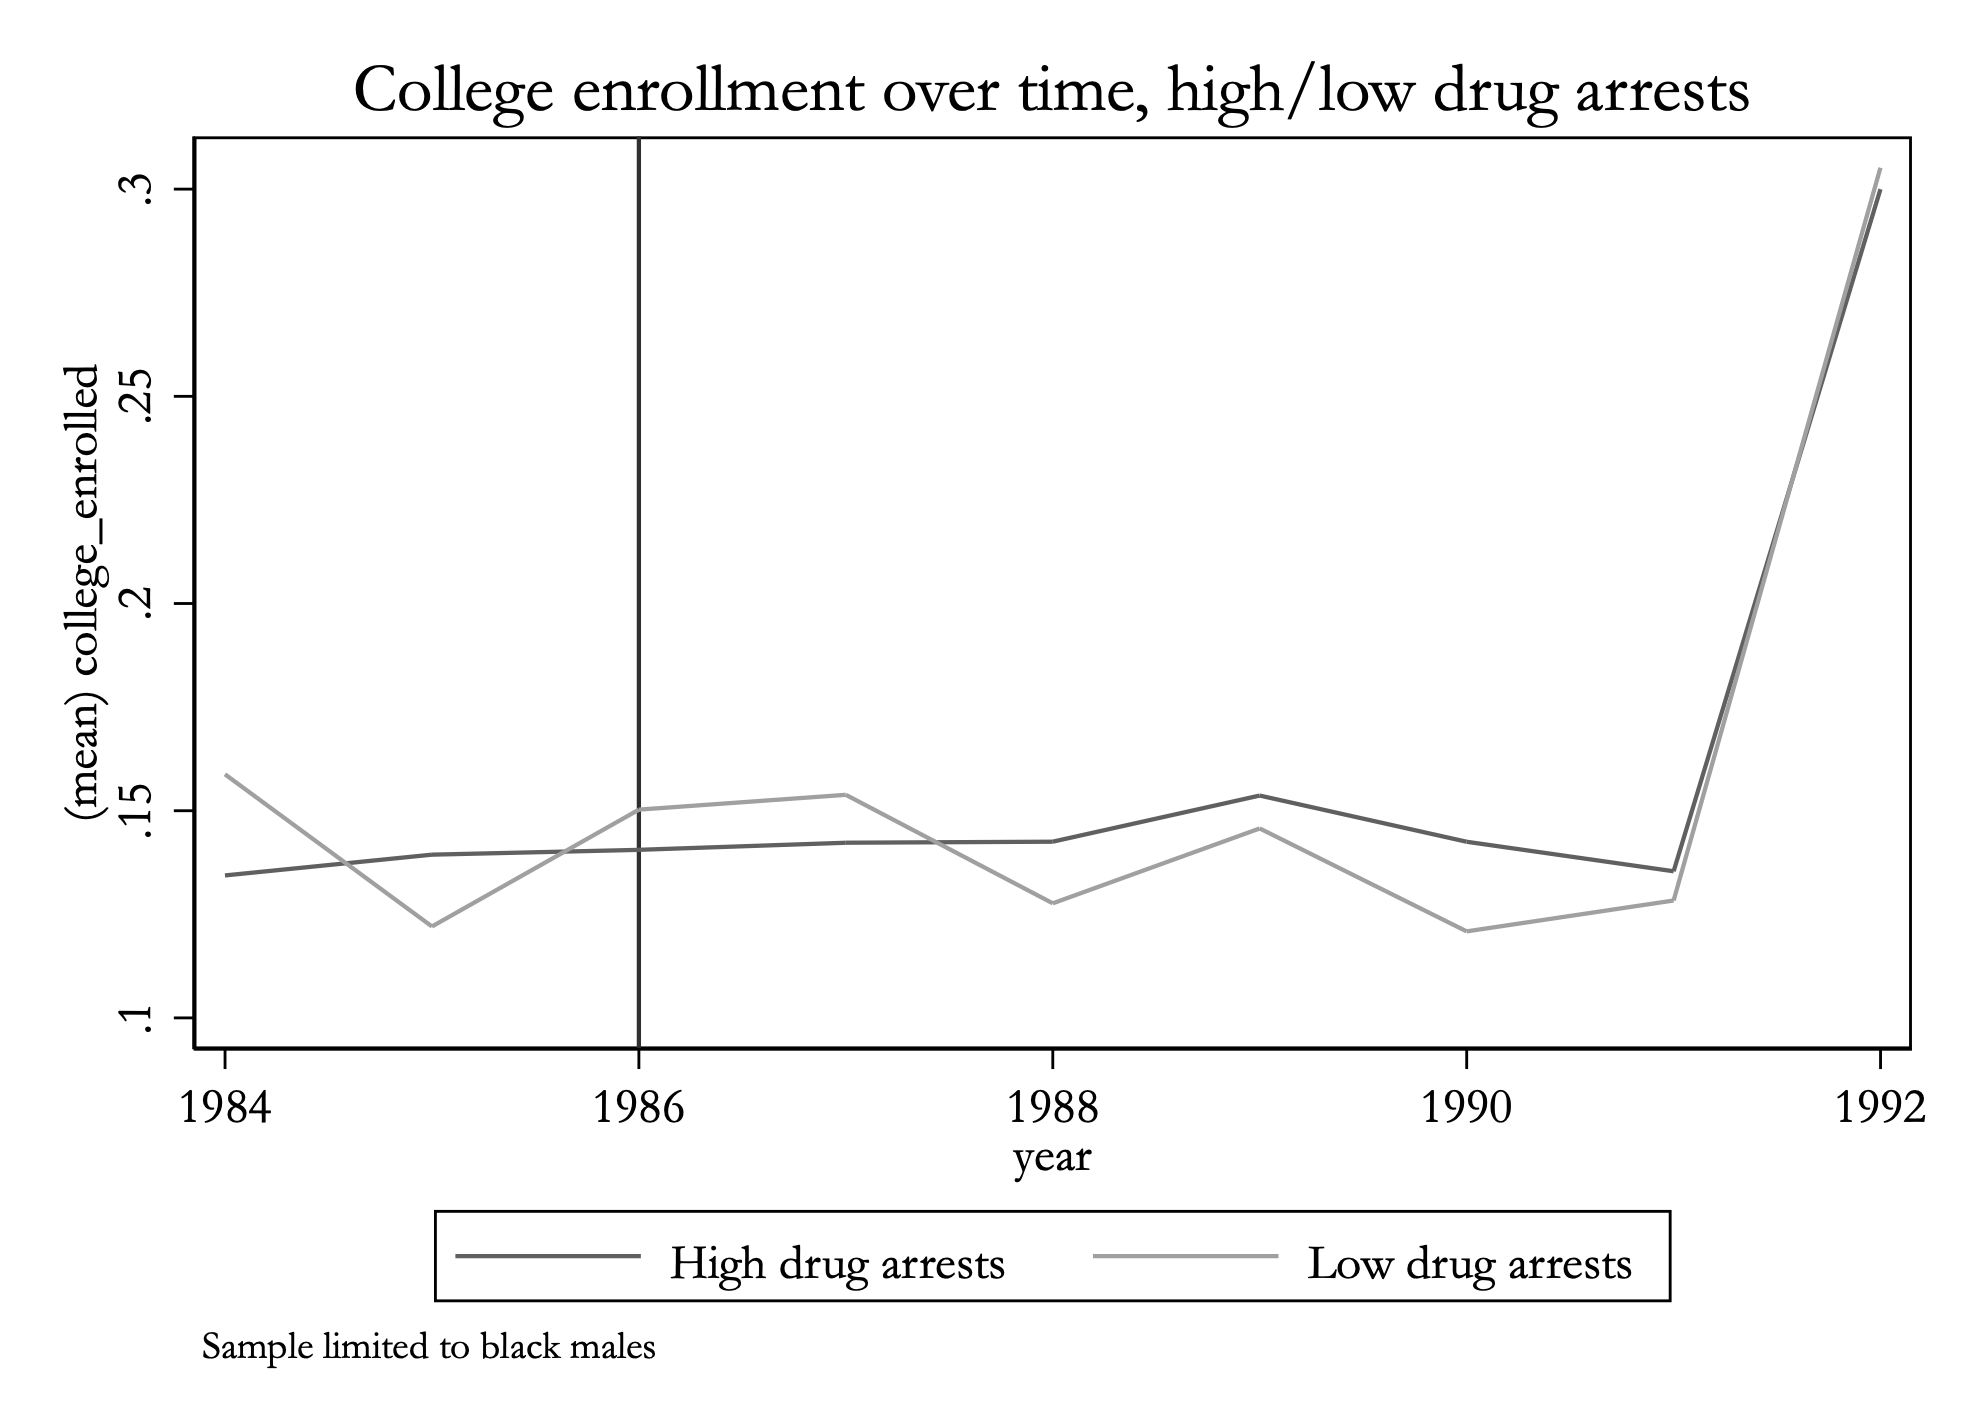
\includegraphics[width=7cm]{pretrends/1986/college_enroll_bydrugarrests_1986.png} }}%
    \qquad
    \subfloat[\centering 2010]{{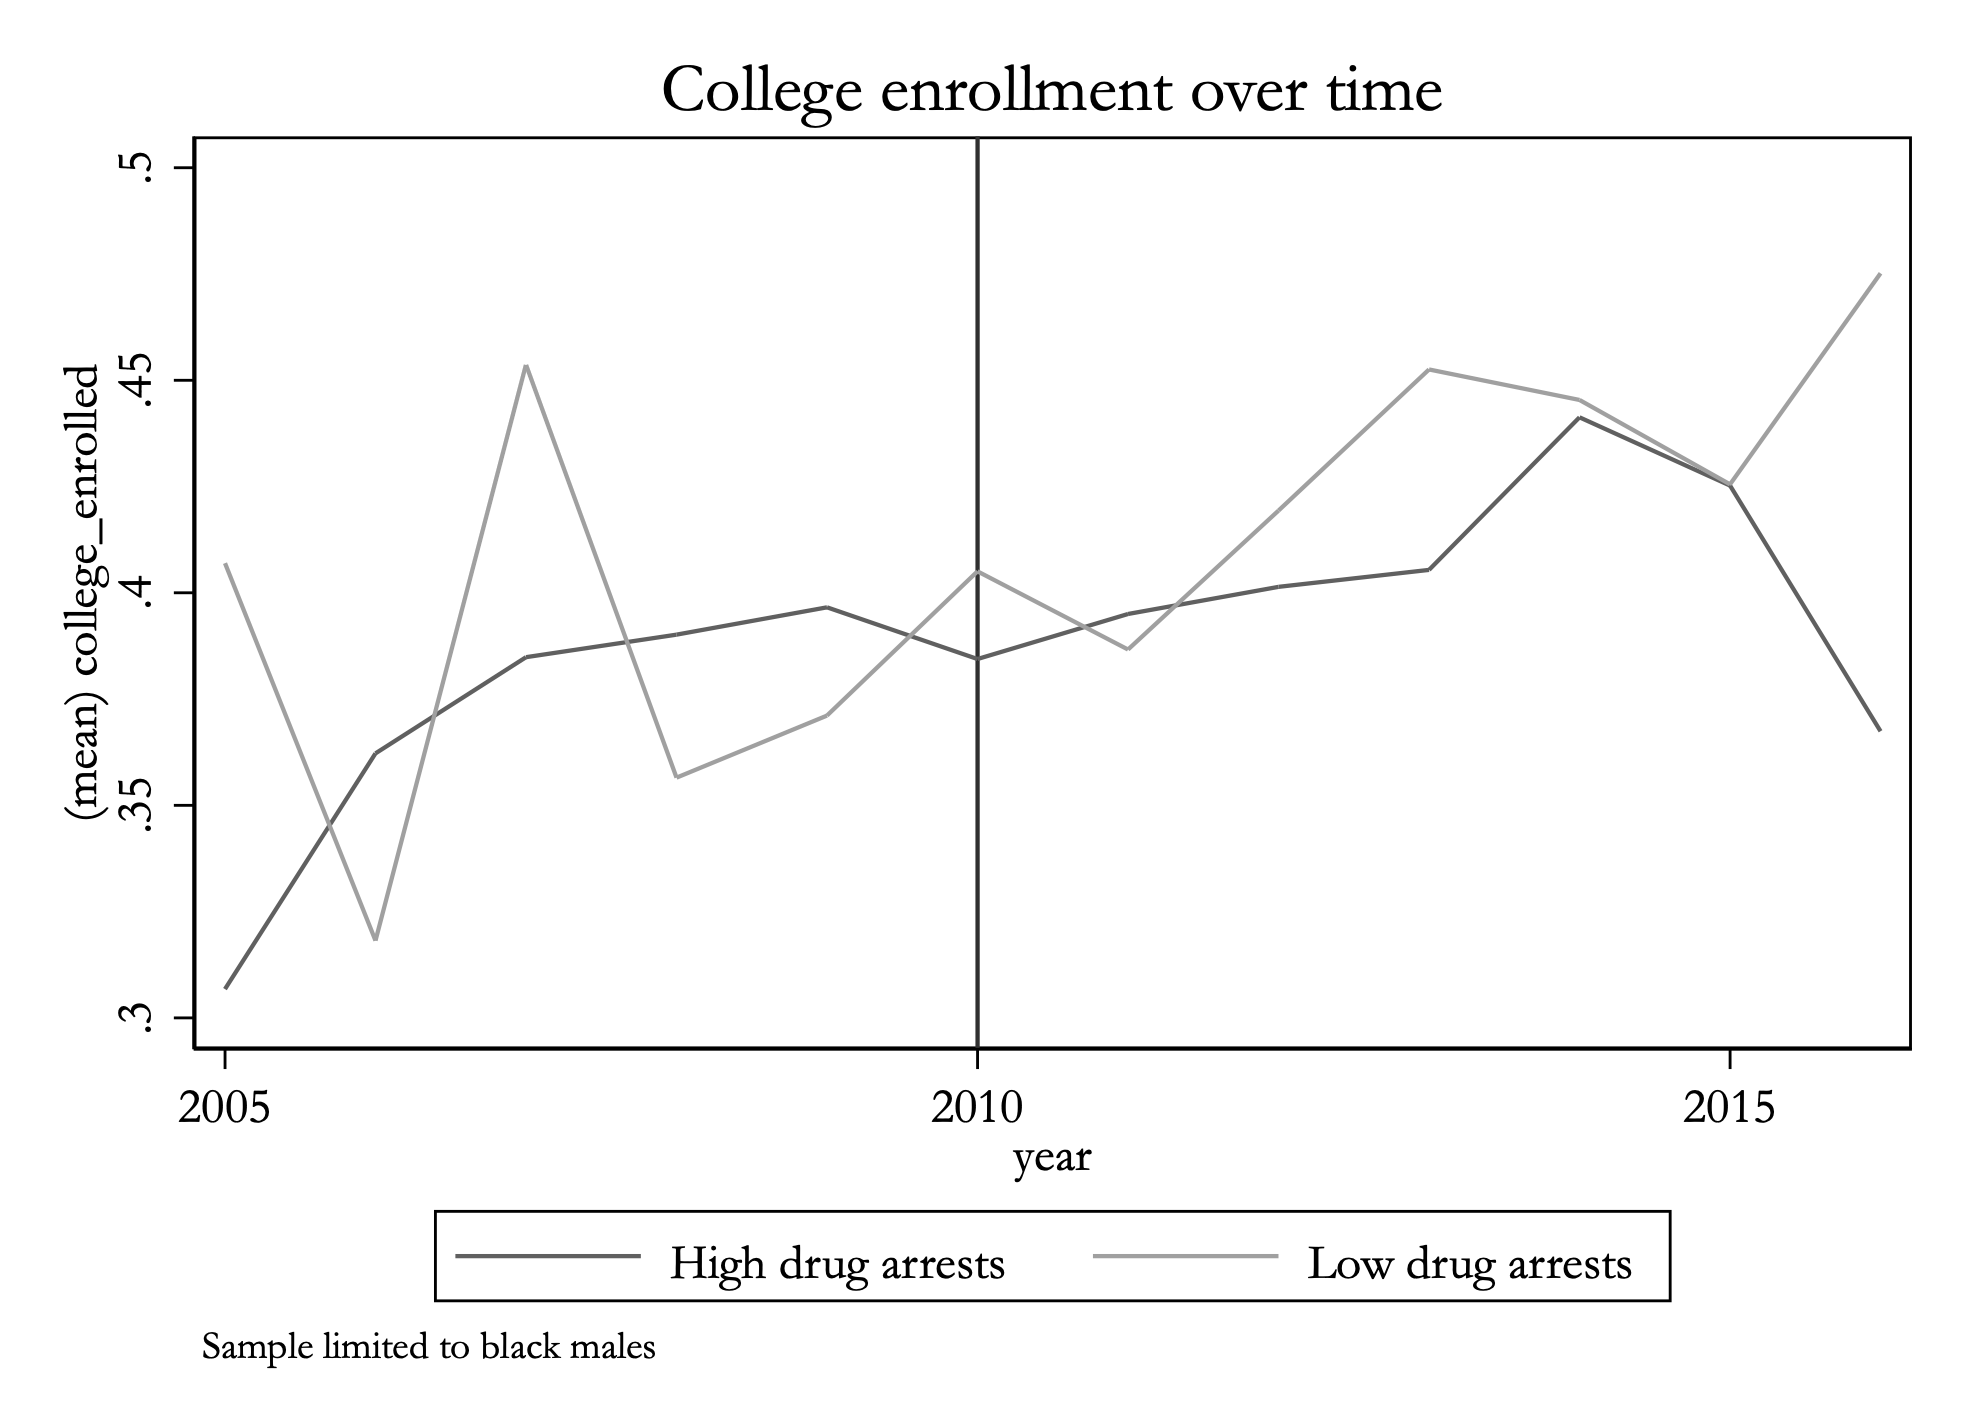
\includegraphics[width=7cm]{pretrends/2010/college_enroll_bydrugarrests_2010.png} }}%
    \label{fig:raw_college_highlowab_1986}%
  \end{figure}
  \begin{figure}[h]
    \centering
    \caption{College Enrollment By States with High vs Low Black Juvenile Drug Arrest Rates}%
    \subfloat[\centering 1986]{{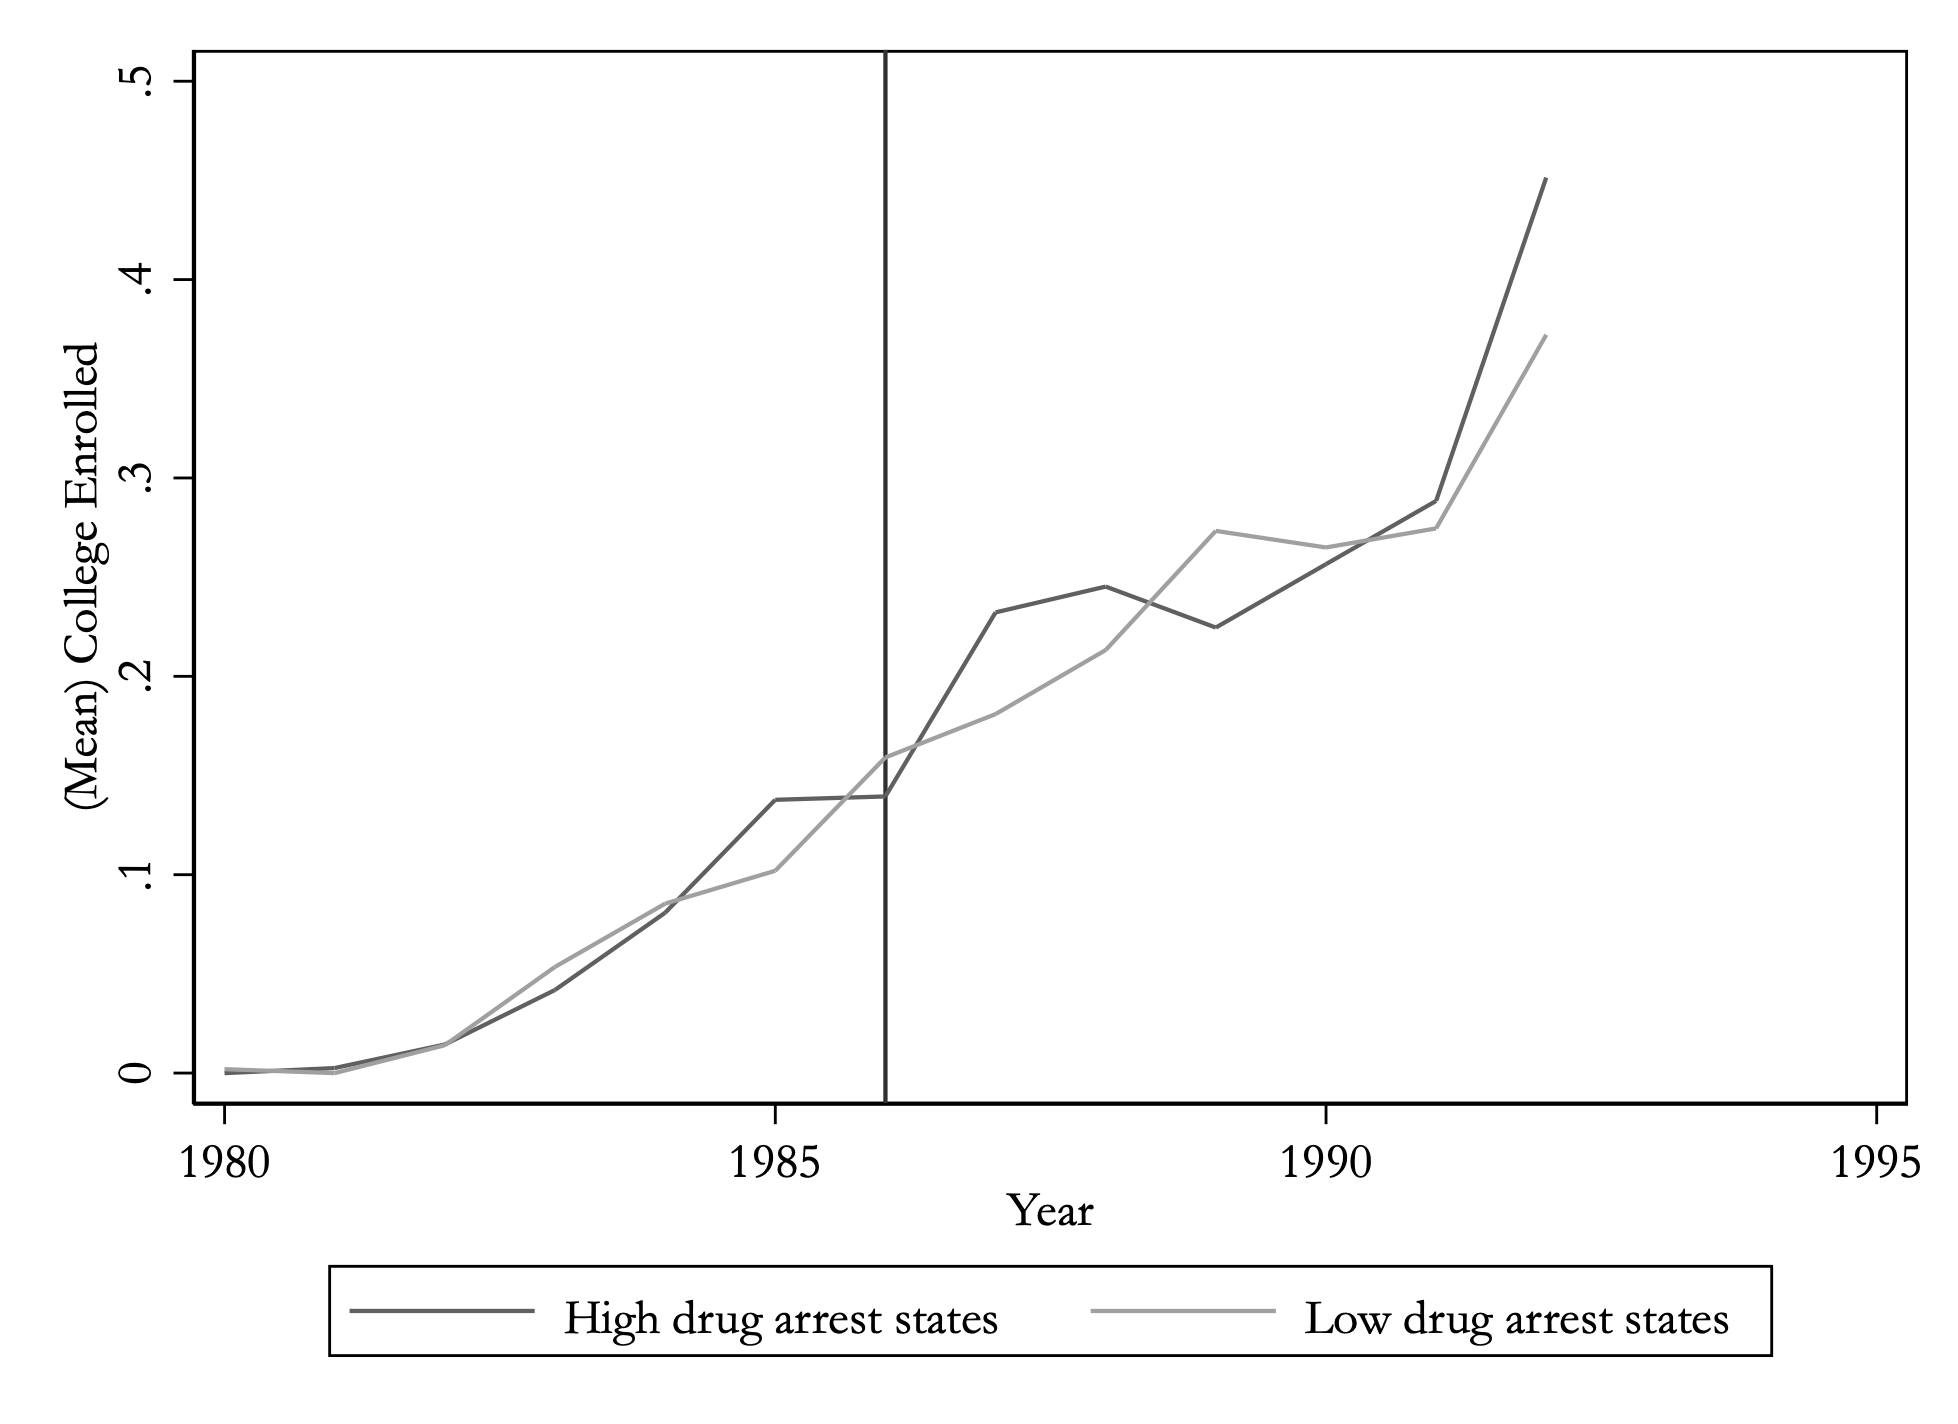
\includegraphics[width=7cm]{pretrends/1986/college_enroll_bydrugarrests_jb_1986.png} }}%
    \qquad
    \subfloat[\centering 2010]{{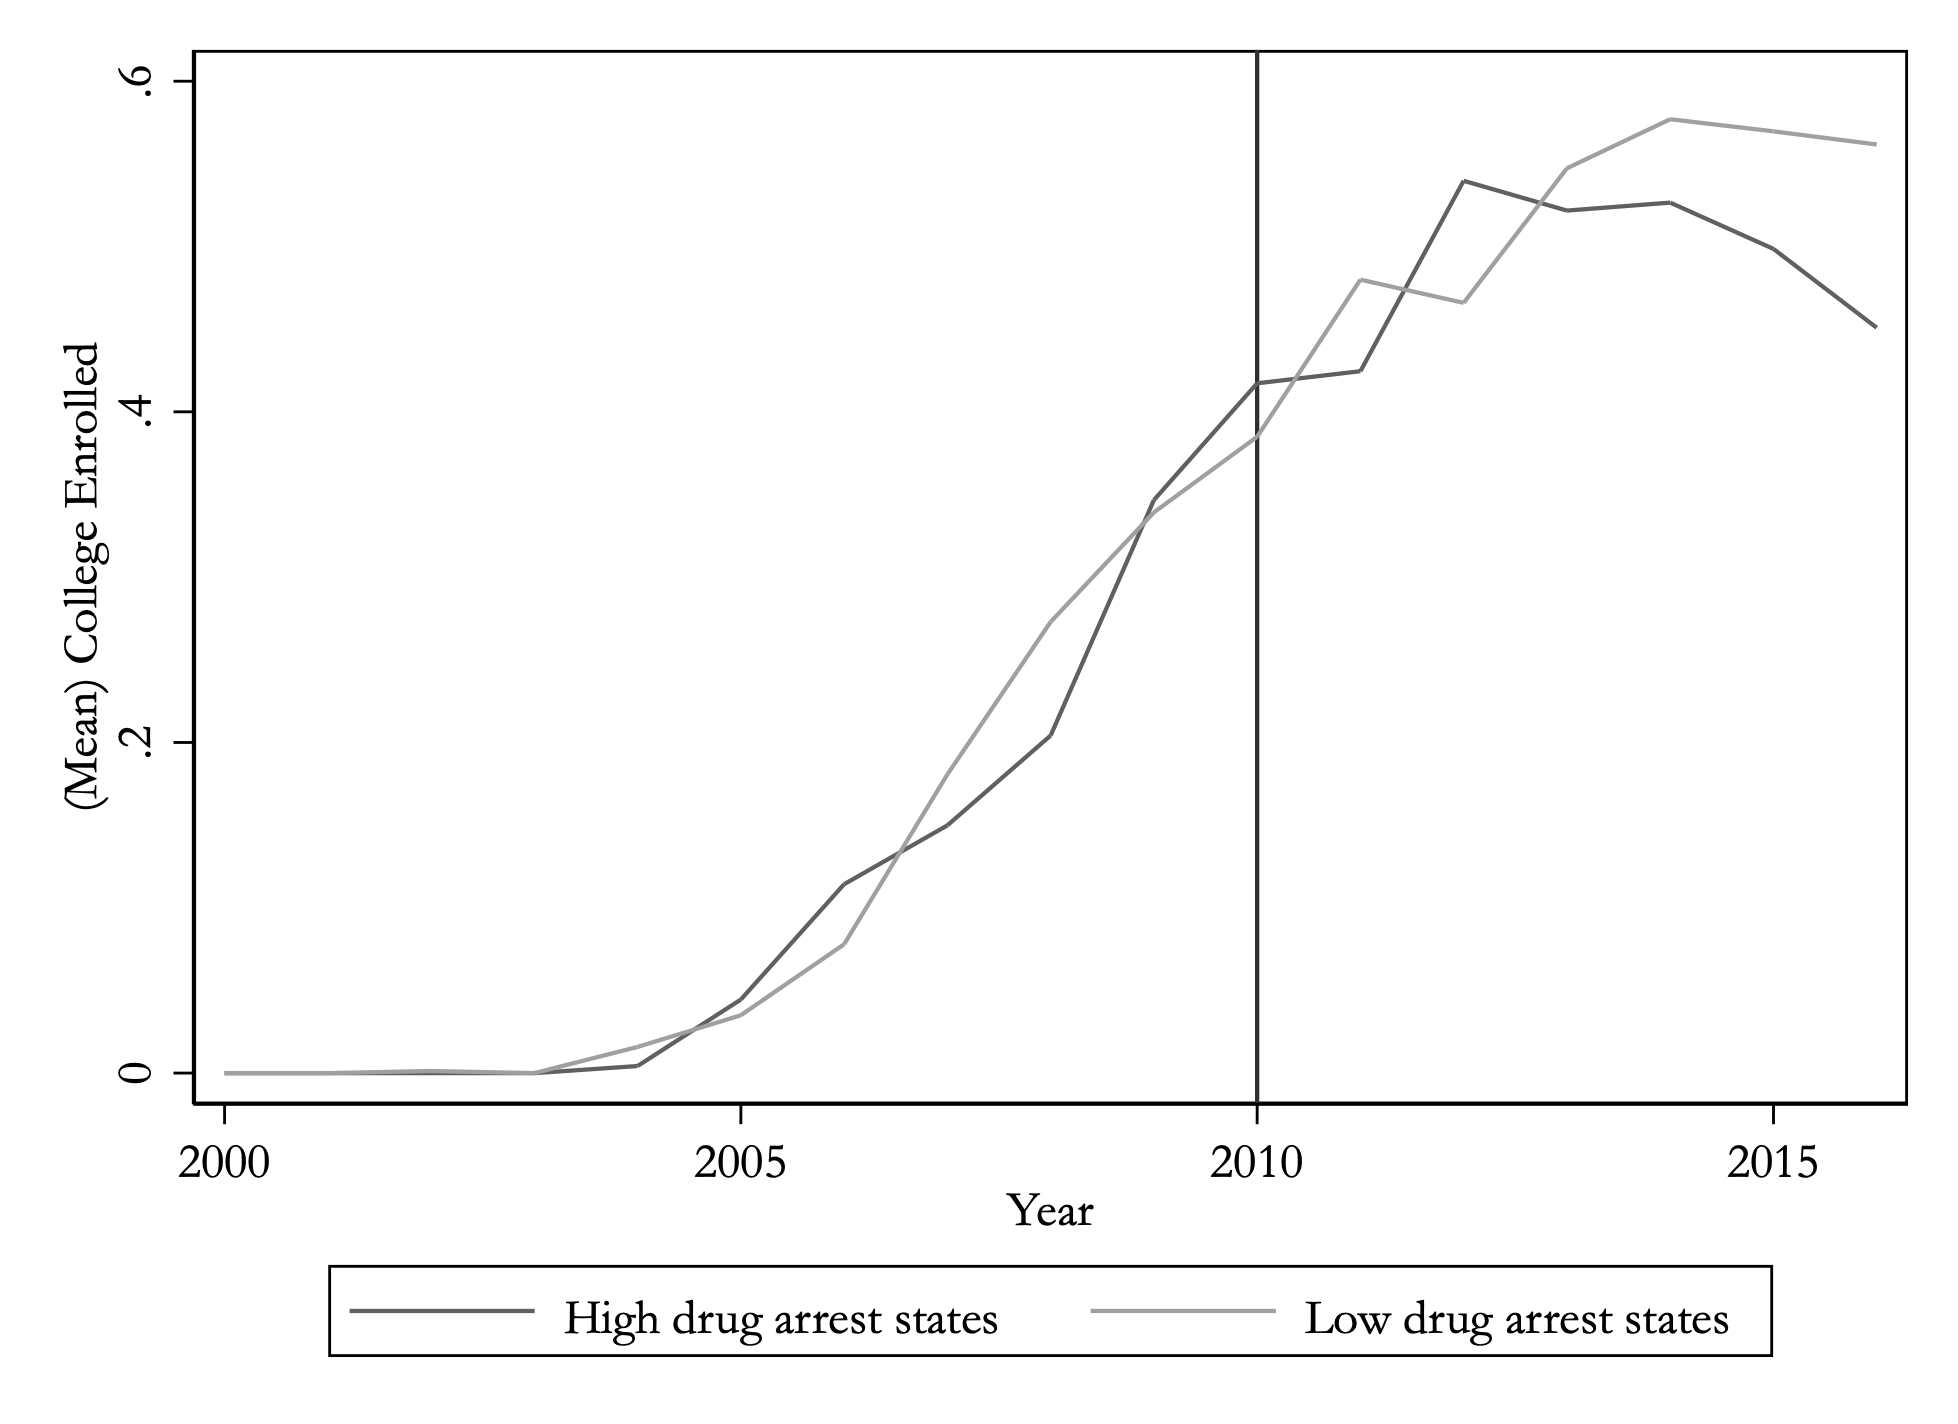
\includegraphics[width=7cm]{pretrends/2010/college_enroll_bydrugarrests_jb_2010.png} }}%
    \label{fig:raw_college_highlowjb_1986}%
  \end{figure}
  
  \begin{footnotesize}
    \noindent Note: These figures report the proportion enrolled in college plotted over time using CPS data from 1984-1992 and 2005-2016 for high black adult/juvenile drug arrest states and low black adult/juvenile drug arrest states, where high black adult/juvenile drug arrest states are defined to be those above the 75th percentile in 1984 and 2008. A vertical line is drawn to denote the passage of the Anti-Drug Abuse Act of 1986 and the Fair Sentencing Act of 2010. The sample is defined as black males aged 18-24 in 1986 and 2010 who were not incarcerated at the time of the survey.
  \end{footnotesize}
  
  \clearpage

  \begin{figure}[h]
    \caption{Black Adult Drug-related Arrest Rate Per 100,000 in 1984} 
    \centering
    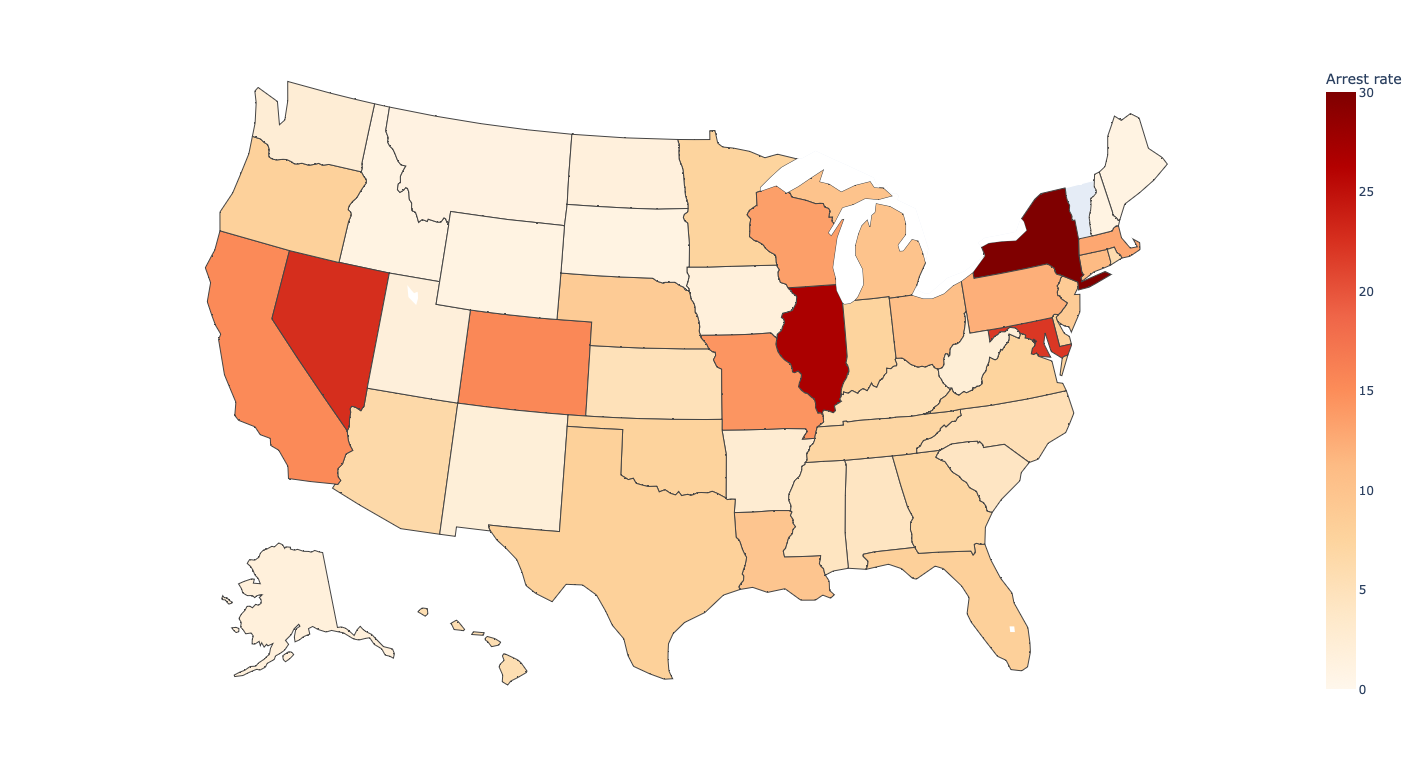
\includegraphics[width=0.8\textwidth]{heatmap/ab1986.png}
    \label{fig:heatmap}
  \end{figure}
  
  \begin{footnotesize}
    \noindent Note: This figure presents a heatmap of the United States at the state level using UCR Program data. The data is from 1984, and I use all drug-related arrests for Black adult men. Although New York's normalized arrest rate is at 48, I capped the maximum at 30 for clarity of states with low normalized drug arrest rates, since the distribution is heavily right-skewed. High drug arrest states are defined as states above the 75th percentile, and the 75th percentile is at 17.4 Black adult arrests per 100,000.
  \end{footnotesize}
  
  \vspace*{8mm}
  
  \begin{figure}[h]
    \centering
    \caption{Distribution of Black Adult Drug-Related Arrest Rates}%
    \subfloat[\centering 1984]{{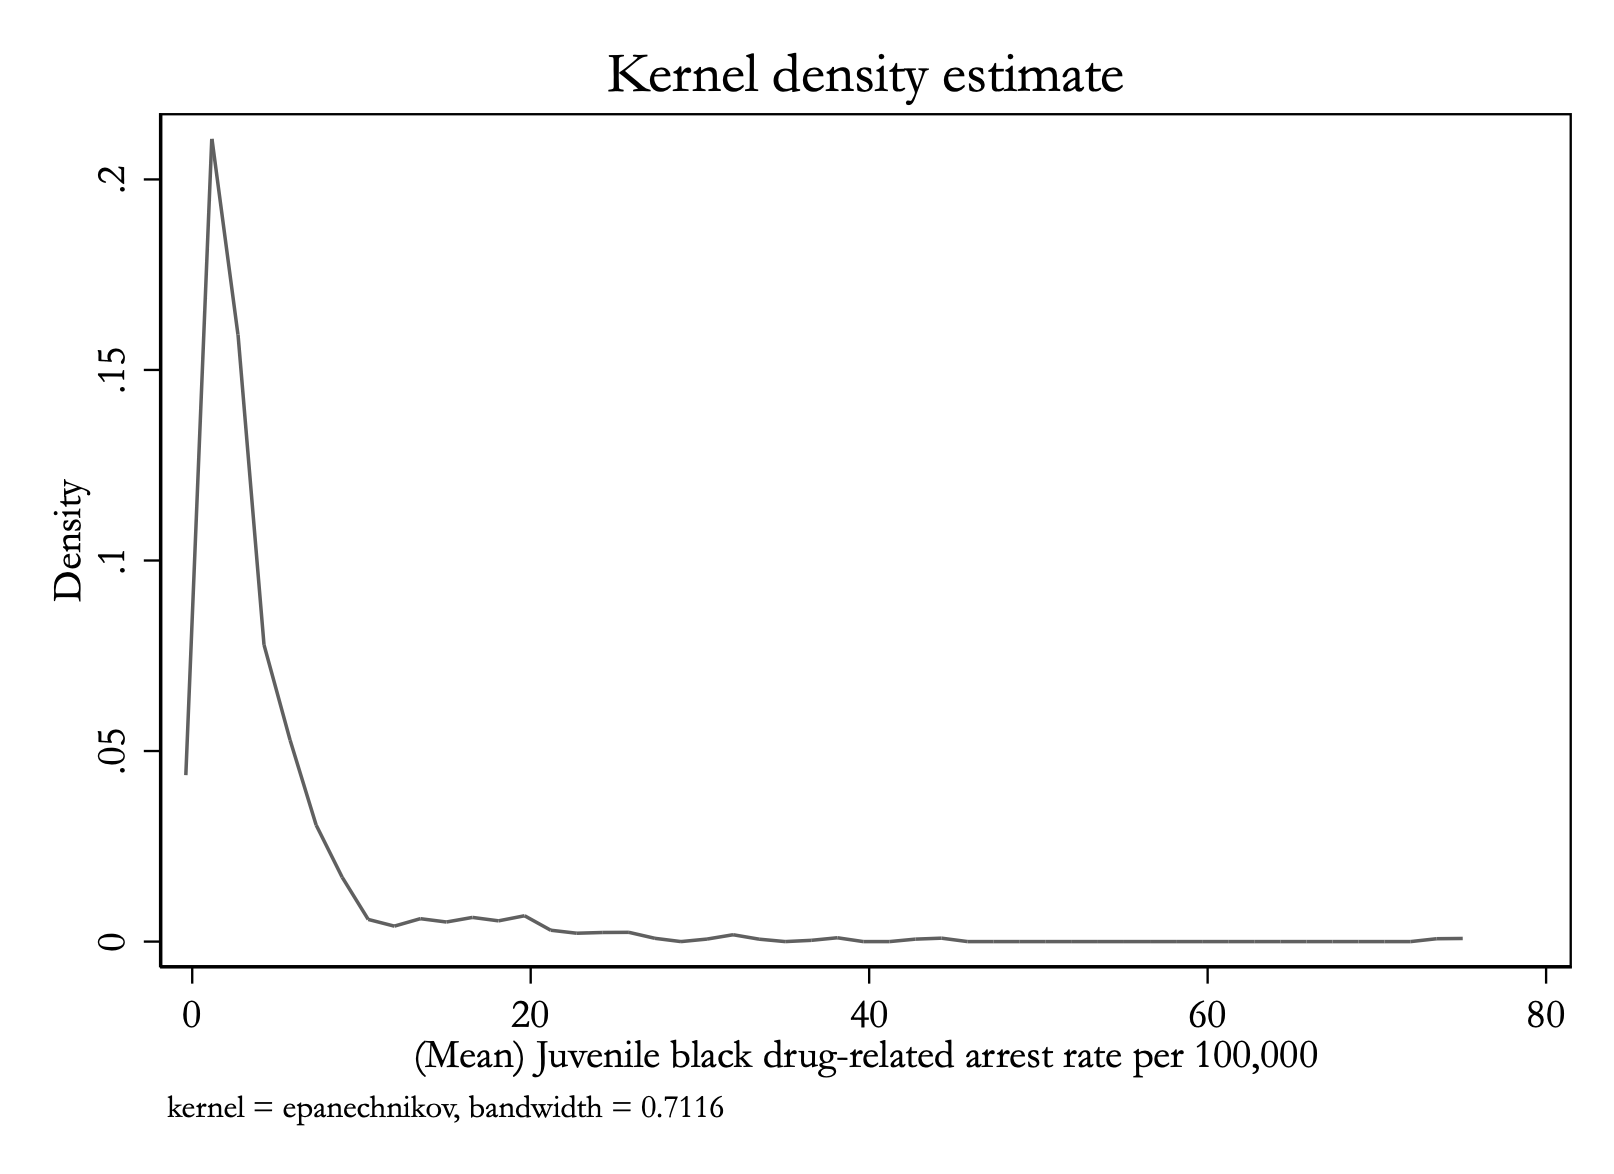
\includegraphics[width=7cm]{descriptive/norm_jb_100000_density_1986} }}%
    \qquad
    \subfloat[\centering 2008]{{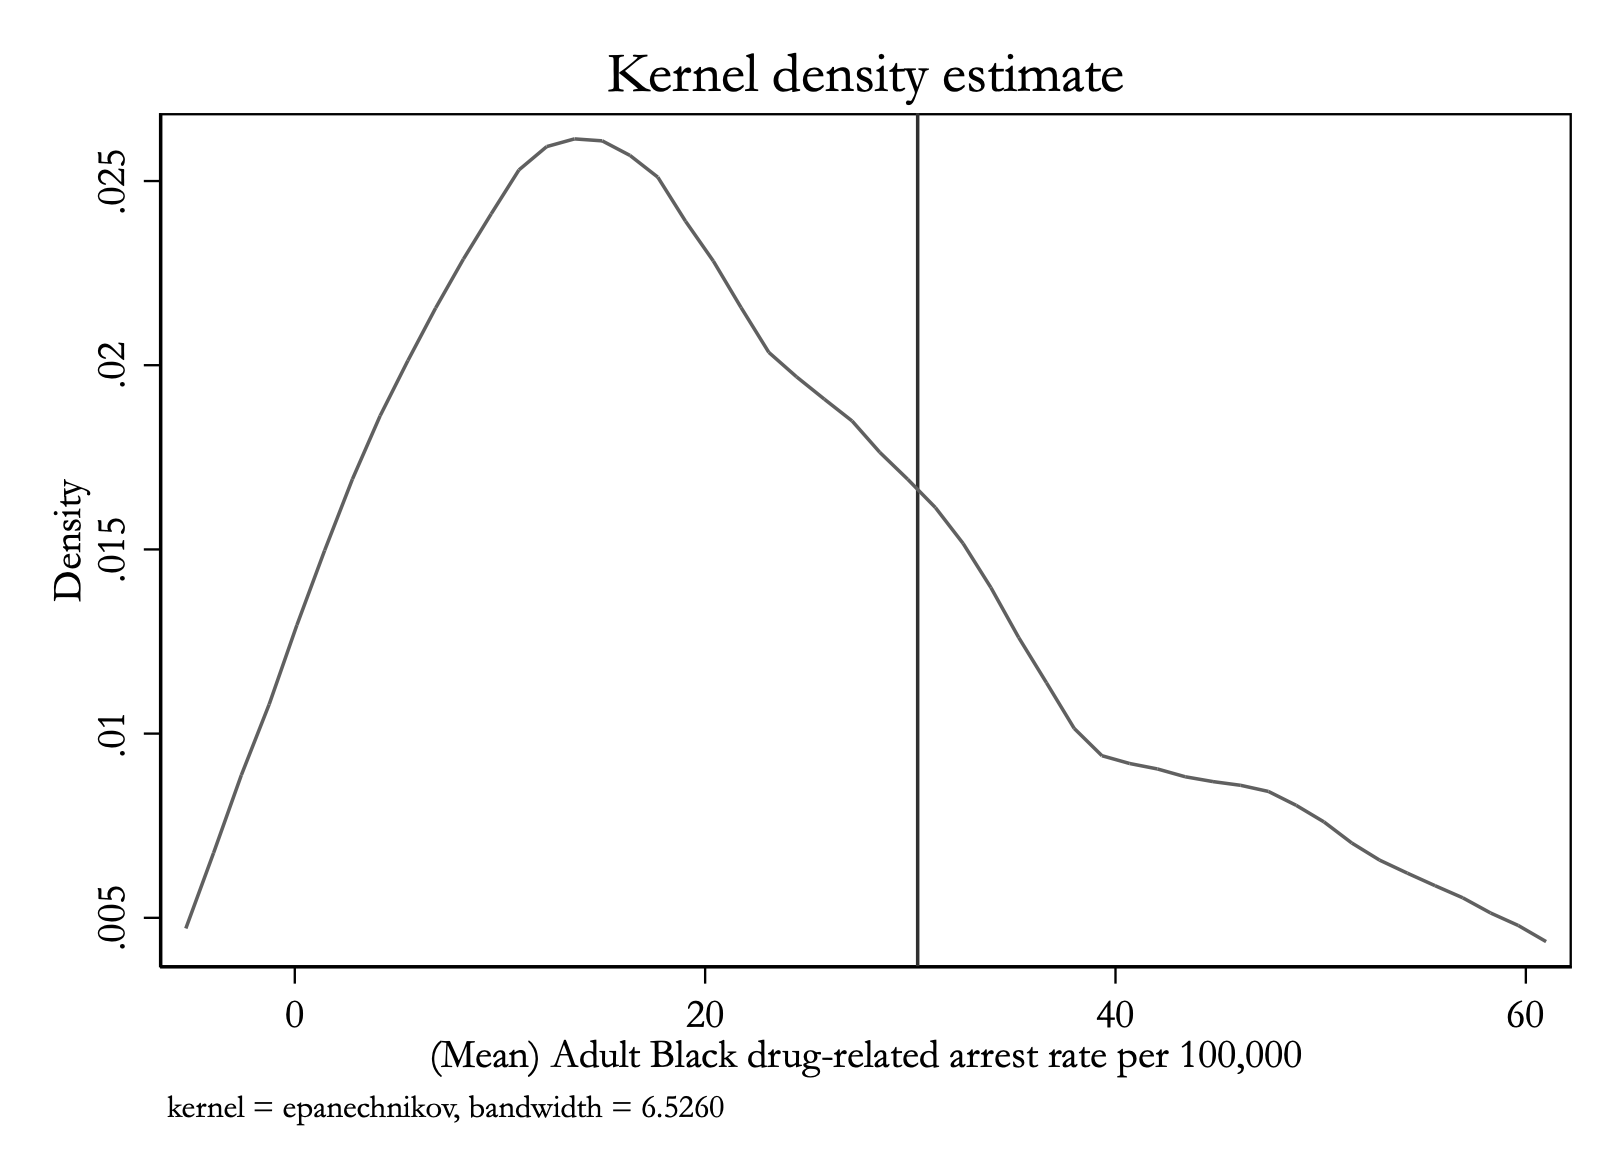
\includegraphics[width=7cm]{descriptive/norm_jb_100000_density_2010.png} }}%
    \label{fig:density_jb}%
  \end{figure}
  \begin{footnotesize}
    \noindent Note: These figures report the kernel density estimates for the normalized drug-related Black adult arrest rate in 1984 and 2008. The vertical line denotes the 75th percentile. Right tail outliers were winsorized at the 95\% level for both figures.
  \end{footnotesize}
  
  \clearpage
     

  % Event study
  \begin{figure}[h]
    \caption{Effect of Anti-Drug Abuse Act on Drug-related Arrest Rate of Adult Black Men, Comparing States with High and Low Black Adult Drug-Related Arrest Rates (with Fixed Effects)}
    \centering
    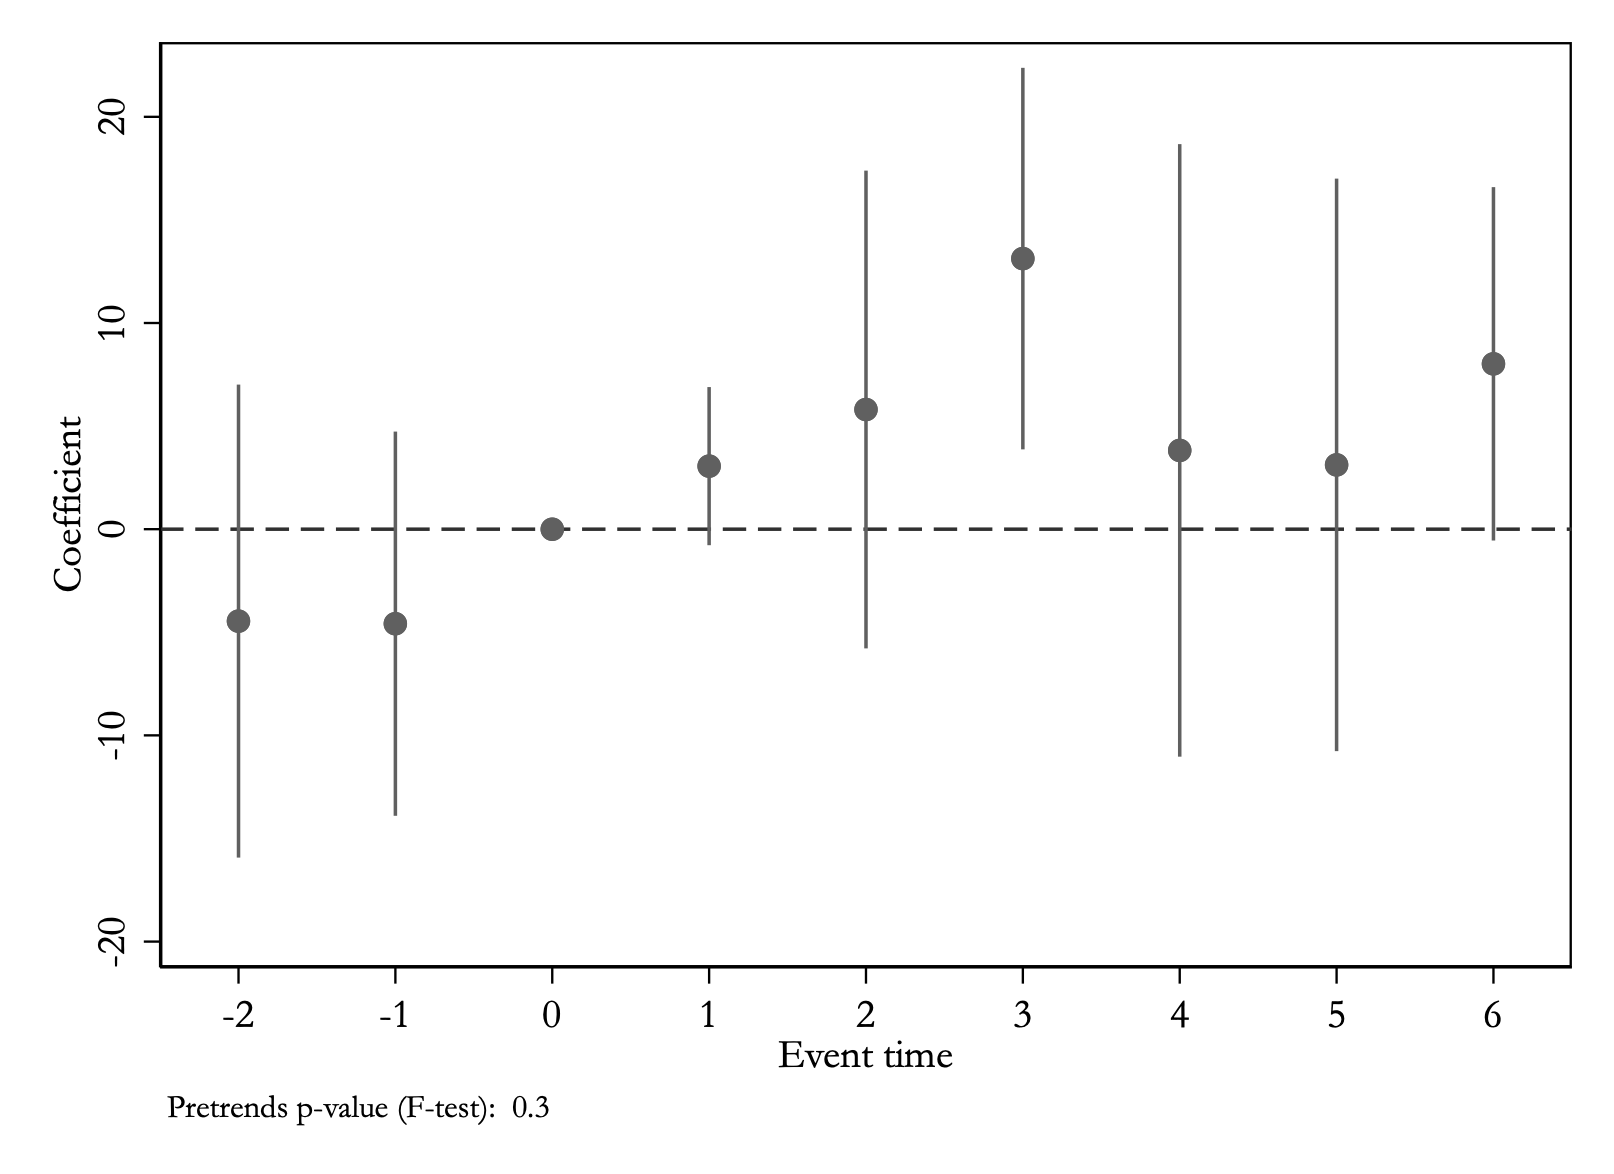
\includegraphics[width=0.7\textwidth]{eventstudy/high_drug_use/high_drug_eventstudy_1986.png}
    \label{fig:ab_es_1986}
  \end{figure}

  \begin{figure}[H]
    \caption{Effect of Anti-Drug Abuse Act on Drug-related Arrest Rate of Adult Black Men, Comparing States with High and Low Black Adult Drug-Related Arrest Rates (without Fixed Effects)}
    \centering
    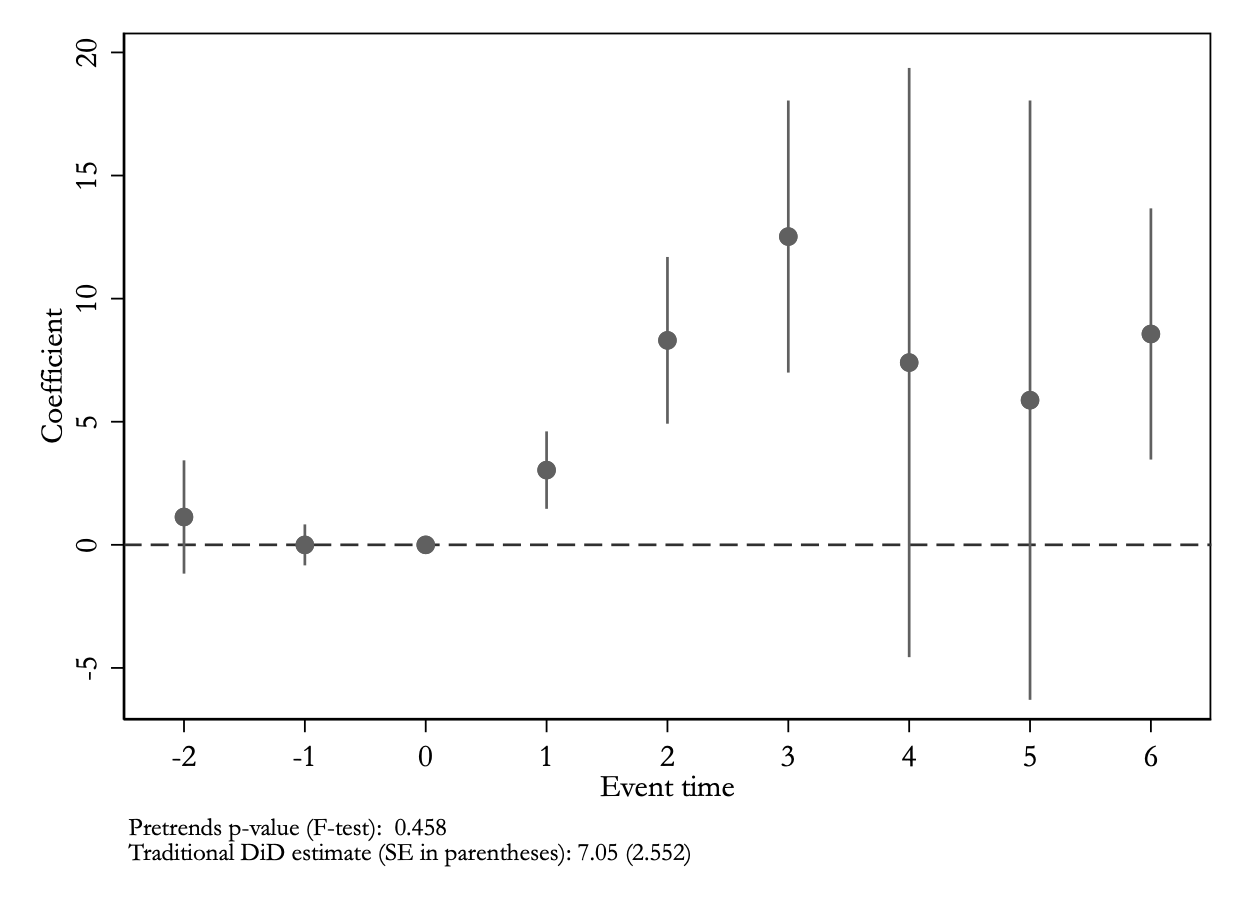
\includegraphics[width=0.7\textwidth]{eventstudy/high_drug_use/high_drug_eventstudy_nofe_1986.png}
    \label{fig:ab_es_1986_nofe}
  \end{figure}
  
  \begin{footnotesize}
    \noindent Note: This figure reports coefficients from the estimation of equation \ref{eq:state_level_es} evaluating the impact of the Anti-Drug Abuse Act of 1986 on arrest rates per 100,000 related to drug violations using CPS and UCR data from 1982-1992. Event time $0 \coloneqq 1986$. The coefficients represent the change in outcomes for high-drug arrest states relative to non-high-drug arrest states, where high black adult drug arrest states are defined to be those above the 75th percentile in 1984. The sample is defined as black males aged 18-24 in 1986 who were not incarcerated at the time of the survey. Control variables include population and unemployment rates at the state-year level. Right tail arrest rate outliers were winsorized at the 95\% level.
  \end{footnotesize}
  
  \clearpage

  \begin{figure}[h]
    \caption{Effect of Anti-Drug Abuse Act on Drug-related Arrest Rate of Black Men, Comparing States with High and Low Black Juvenile Drug-Related Arrest Rate}
    \centering
    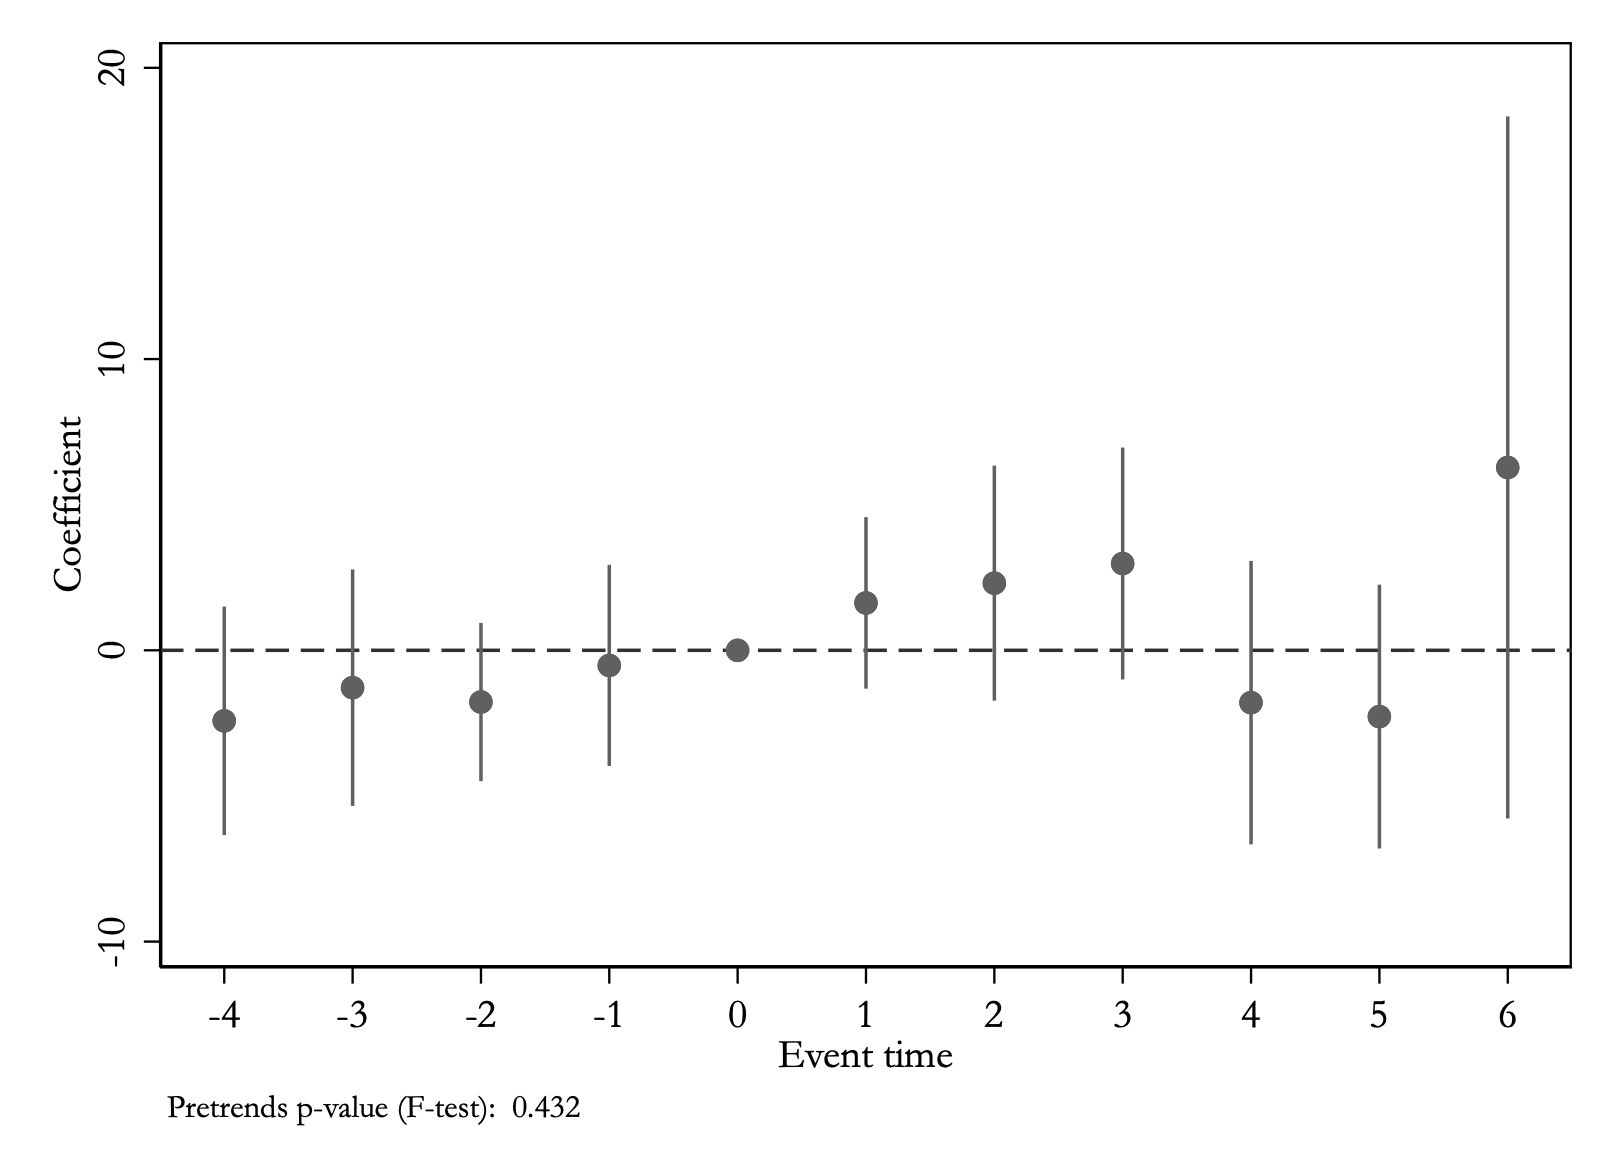
\includegraphics[width=1\textwidth]{eventstudy/high_drug_use/high_drug_eventstudy_1986_jb.png}
    \label{fig:jb_es_1986}
  \end{figure}

  \begin{footnotesize}
    \noindent Note: This figure reports coefficients from the estimation of equation 1 evaluating the impact of the Anti-Drug Abuse Act of 1986 on arrest rates per 100,000 related to drug violations using CPS and UCR data from 1982-1992. Event time $0 \coloneqq 1986$. The coefficients represent the change in outcomes for high black juvenile drug arrest states relative to non-high-drug arrest states, where high-drug arrest states are defined to be those above the 75th percentile in 1984. The sample is defined as black males aged 18-24 in 1986 who were not incarcerated at the time of the survey. Control variables include population and unemployment rates at the state-year level. 
  \end{footnotesize}

  \clearpage

  \begin{figure}[h]
    \centering
    \caption{Additional Pre-trend Testing for Coefficients from Figure 7}%
    \subfloat[\centering Linear pre-trend]{{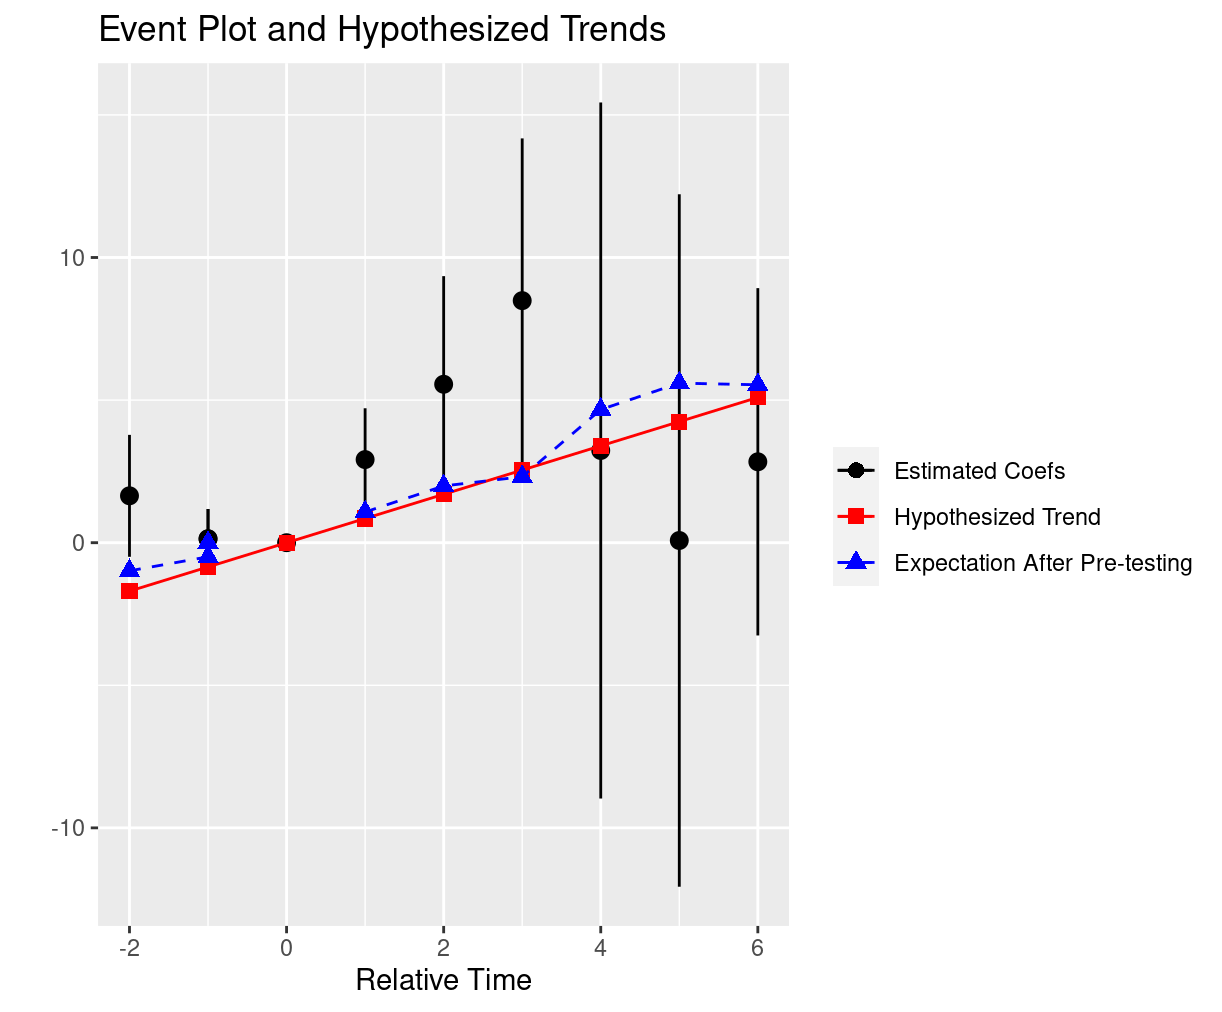
\includegraphics[width=7cm]{pretrends/power/firststage_linear_ab1986.png} }}%
    \qquad
    \subfloat[\centering Quadratic pre-trend]{{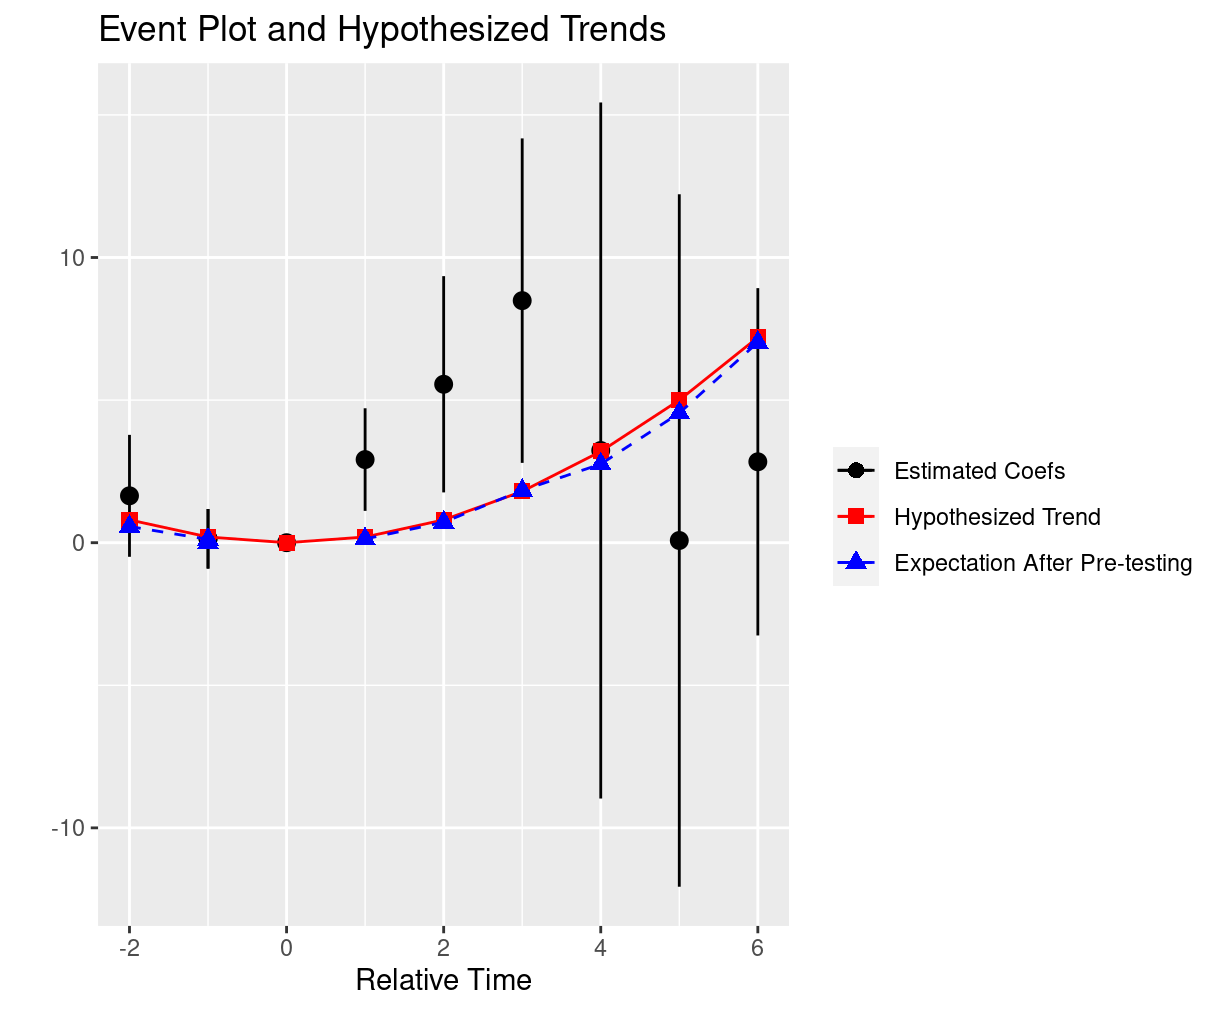
\includegraphics[width=7cm]{pretrends/power/firststage_quad_ab1986.png} }}%
    \label{fig:pre-trends_roth}%
  \end{figure}

  \begin{footnotesize}
    \noindent Note: These two figures were constructed using an R package written by Roth (2022). The figures and pre-trend statistics were calculated using the estimated coefficients from Figure 7 and their corresponding covariance matrixes. The slope in Figure A was constructed such that the power would be about 0.5, while the quadratic trend in Figure B was chosen visually. The blue expectation after pretesting coefficients represents the expected value of the coefficients conditional on passing the pre-test under the hypothesized trend.

    Figure A statistics: 1) power = 0.499, 2) Bayes Factor = 0.549, 3) likelihood ratio = 0.033.

    Figure B statistics: 1) power = 0.155, 2) Bayes Factor = 0.928, 3) likelihood ratio = 2.323.
  \end{footnotesize}

  \clearpage
  
  \begin{figure}[h]
    \centering
    \caption{Effect of Fair Sentencing Act on Drug-related Arrest Rate of Adult Black Men, Comparing High and Low-Intensity States}%
    \subfloat[\centering Using adults arrests]{{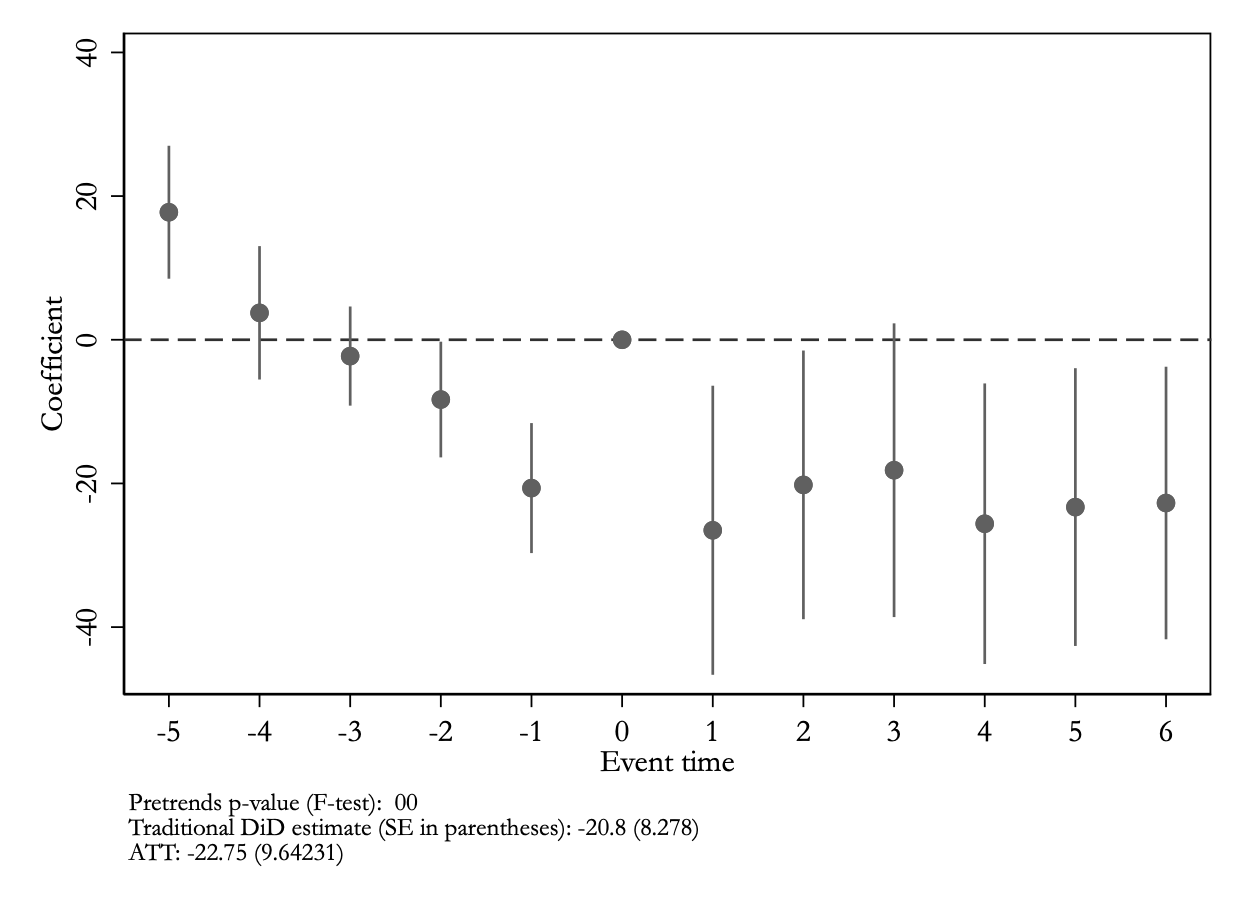
\includegraphics[width=7cm]{eventstudy/high_drug_use/high_drug_eventstudy_2010_ab.png} }}%
    \qquad
    \subfloat[\centering Using juvenile arrests]{{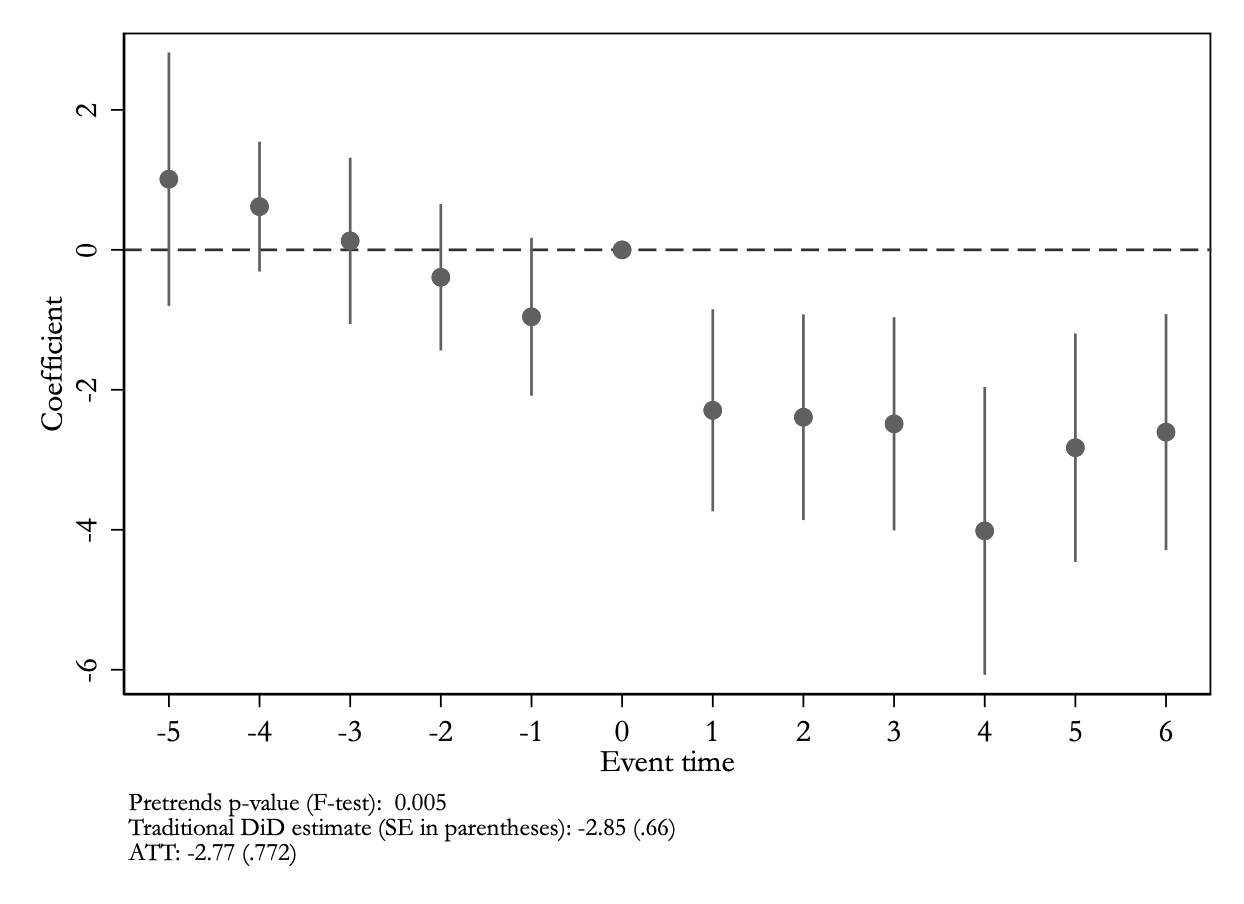
\includegraphics[width=7cm]{eventstudy/high_drug_use/high_drug_eventstudy_2010_jb.png} }}%
    \label{fig:fs_es_2010}%
  \end{figure}


  \begin{footnotesize}
    \noindent Note: These figures report coefficients from the estimation of equation 1 evaluating the impact of the Fair Sentencing Act of 2010 on arrest rates per 100,000 related to drug violations using CPS-UCR merged data from 2005-2015. Figure A defines high-intensity states using Black adult arrests, while Figure B defines high-intensity states using Black juvenile arrests. Event time $0 \coloneqq 2010$. The coefficients represent the change in outcomes for high black adult drug arrest states relative to non-high-drug arrest states, where high-drug arrest states are defined to be those above the 75th percentile in 2008. The sample is defined as black males aged 18-24 in 2010 who were not incarcerated at the time of the survey. Control variables include population and unemployment rates at the state-year level. 
  \end{footnotesize}

\clearpage 

\begin{figure}[h]
  \centering
  \caption{Effect of Anti-Drug Abuse Act on the College Enrollment Rate of Adult Black Men, Comparing High and Low-Intensity States}%
  \subfloat[\centering Using adults arrests]{{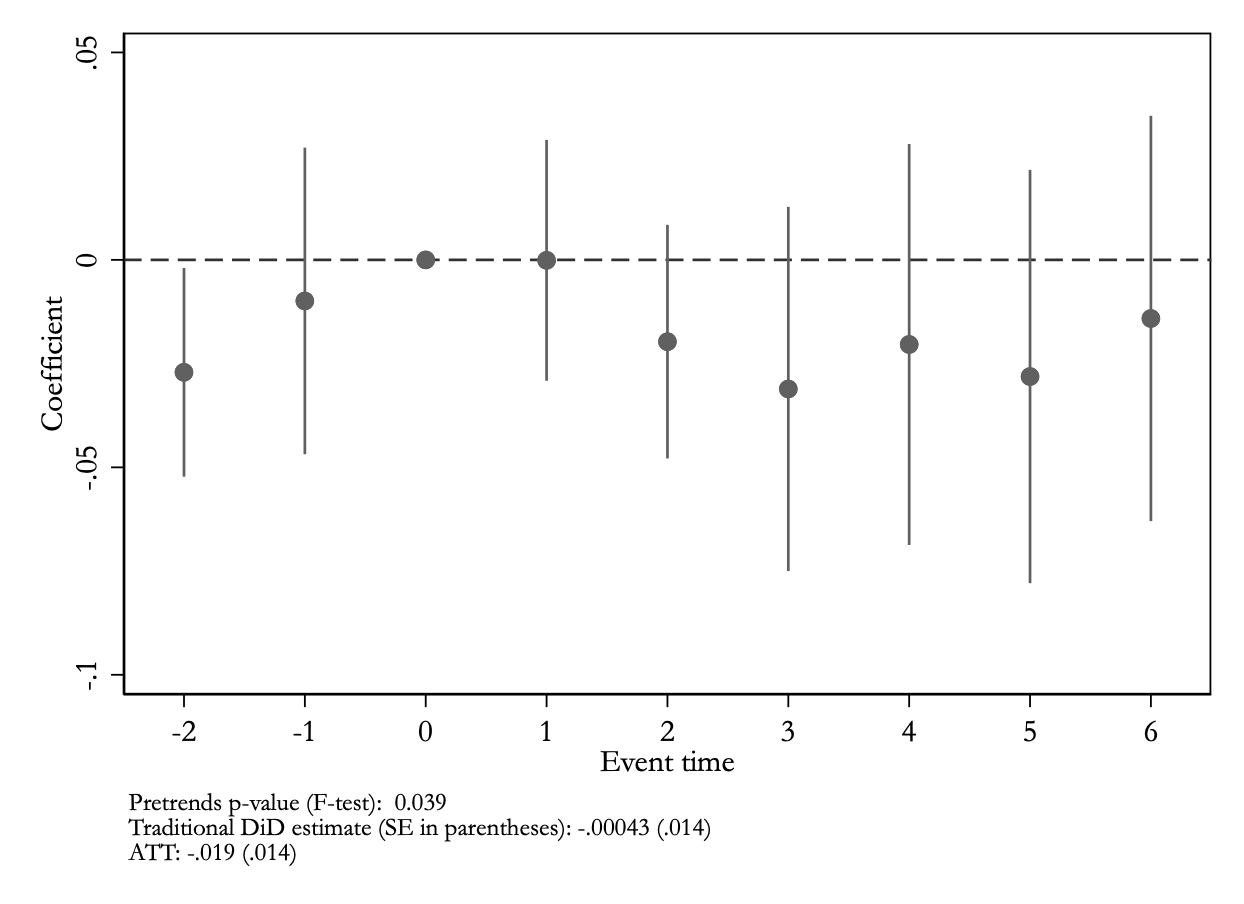
\includegraphics[width=7cm]{eventstudy/high_drug_use/reducedform_ab1986.png} }}%
  \qquad
  \subfloat[\centering Using juvenile arrests]{{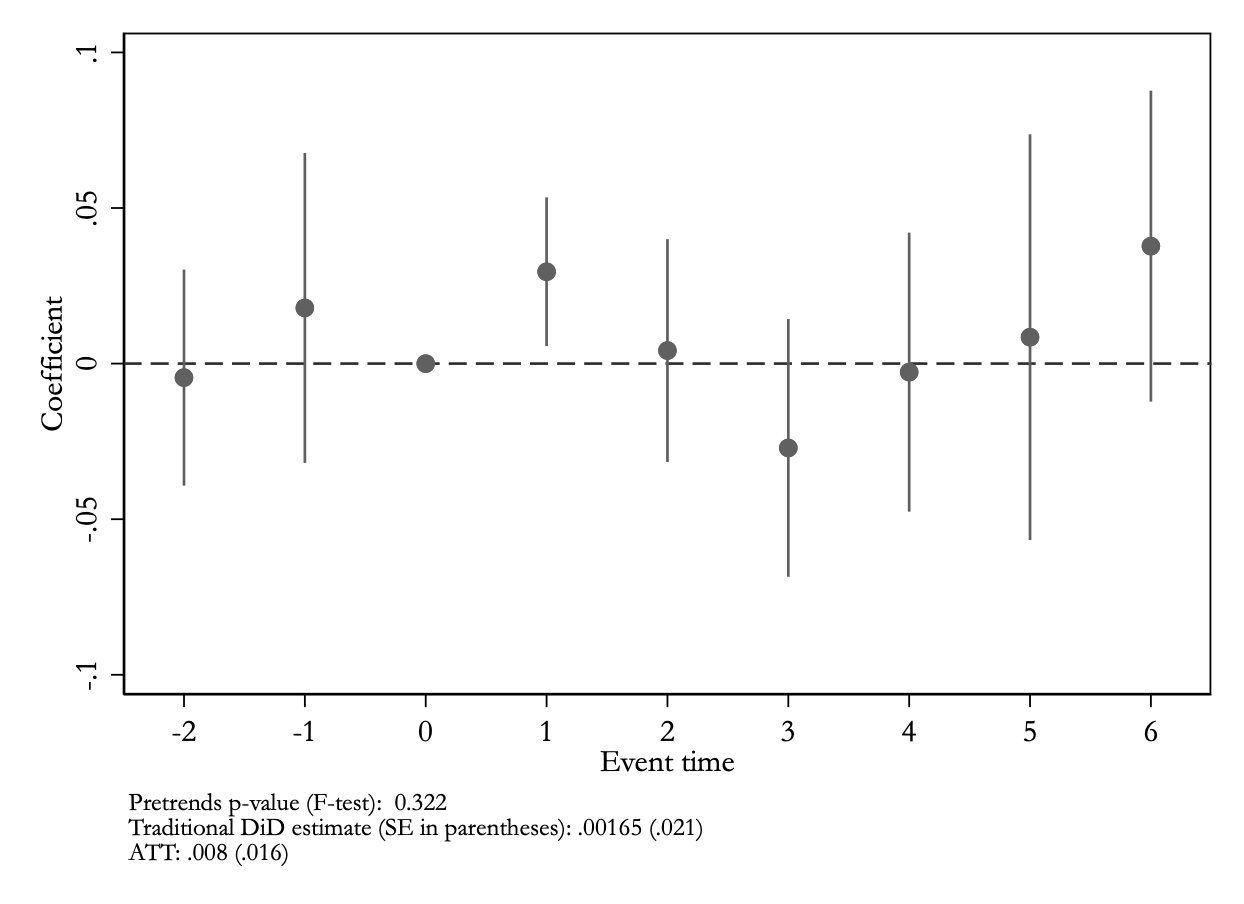
\includegraphics[width=7cm]{eventstudy/high_drug_use/reducedform_jb1986.png} }}%
  \label{fig:rs_es_1986}%
\end{figure}

\begin{footnotesize}
  \noindent Note: These figures report coefficients from the estimation of equation 1 evaluating the impact of the Anti-Drug Abuse Act of 1986 on college enrollment rates using CPS-UCR merged data from 1984-1992. Figure A defines high-intensity states using Black adult arrests, while Figure B defines high-intensity states using Black juvenile arrests. Event time $0 \coloneqq 1986$. The coefficients represent the change in outcomes for high black adult drug arrest states relative to non-high-drug arrest states, where high-drug arrest states are defined to be those above the 75th percentile in 1984. The sample is defined as black males aged 18-24 in 1986 who were not incarcerated at the time of the survey. Control variables include population and unemployment rates at the state-year level. 
\end{footnotesize}

\clearpage

\begin{figure}[h]
  \centering
  \caption{Effect of Fair Sentencing Act on the College Enrollment Rate of Adult Black Men, Comparing High and Low-Intensity States}%
  \subfloat[\centering Using adults arrests]{{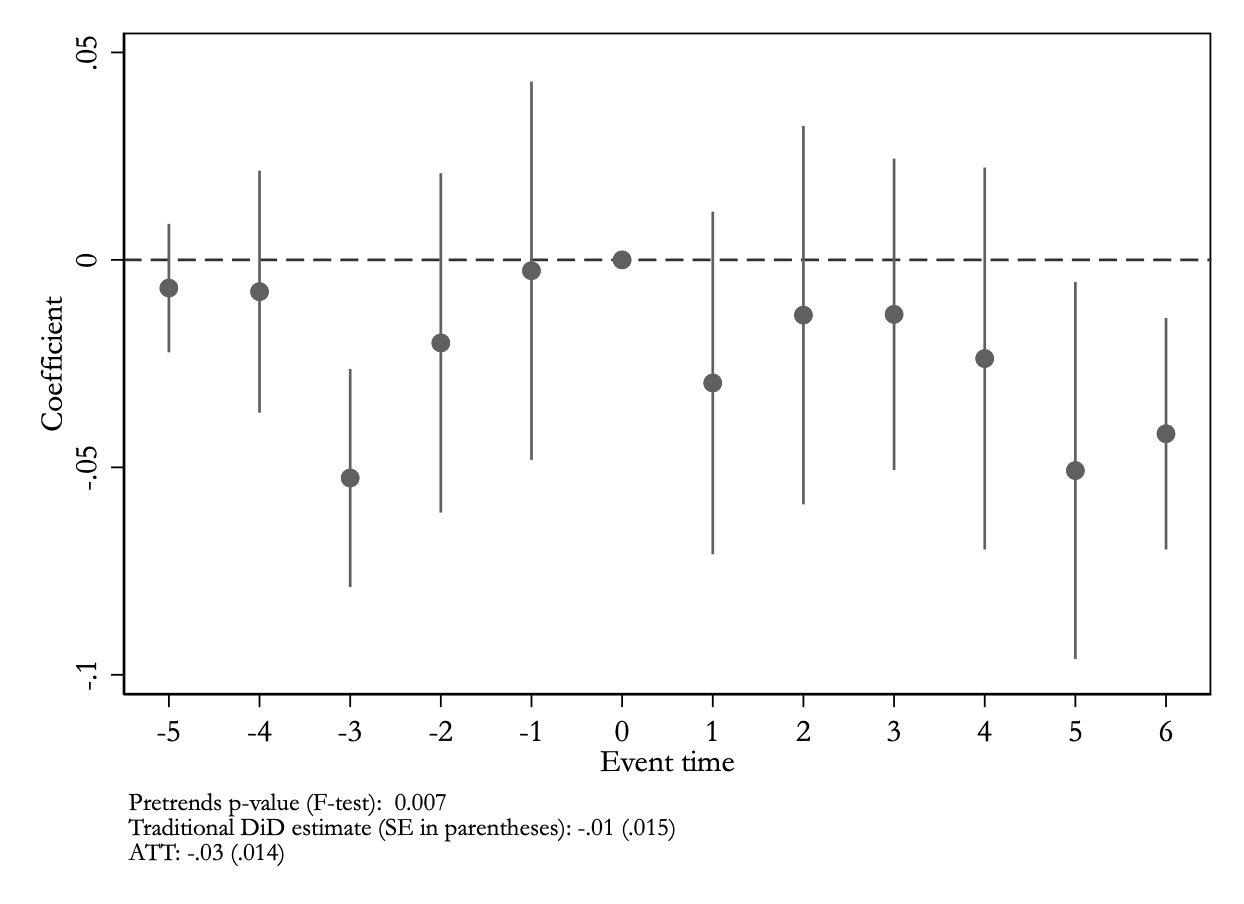
\includegraphics[width=7cm]{eventstudy/high_drug_use/reducedform_ab2010.png} }}%
  \qquad
  \subfloat[\centering Using juvenile arrests]{{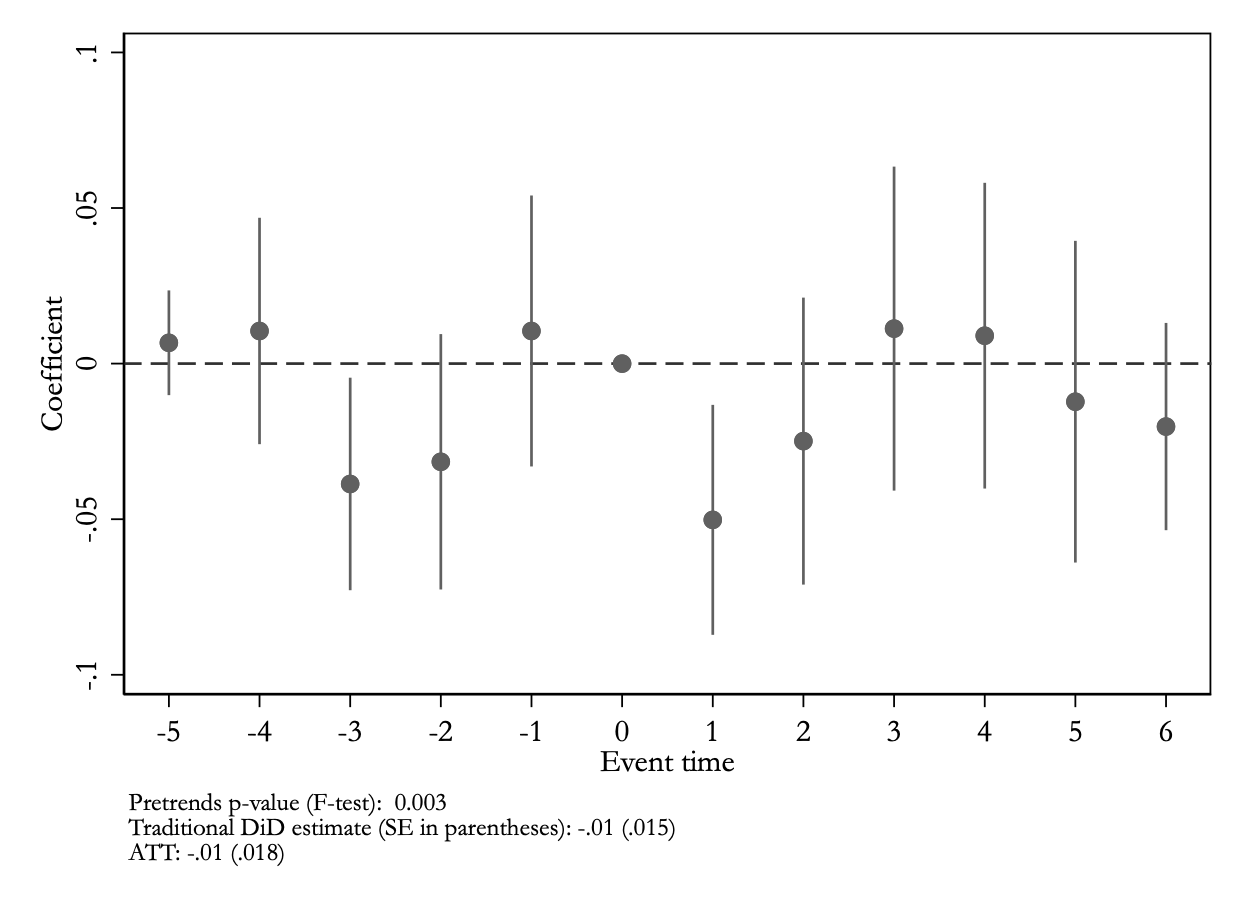
\includegraphics[width=7cm]{eventstudy/high_drug_use/reducedform_jb2010.png} }}%
  \label{fig:rf_jb_es_2010}%
\end{figure}

\begin{footnotesize}
  \noindent Note: These figures report coefficients from the estimation of equation 1 evaluating the impact of the Fair Sentencing Act of 2010 on college enrollment rates using CPS-UCR merged data from 2005-2015. Figure A defines high-intensity states using Black adult arrests, while Figure B defines high-intensity states using Black juvenile arrests. Event time $0 \coloneqq 2010$. The coefficients represent the change in outcomes for high black adult drug arrest states relative to non-high-drug arrest states, where high-drug arrest states are defined to be those above the 75th percentile in 2008. The sample is defined as black males aged 18-24 in 2010 who were not incarcerated at the time of the survey. Control variables include population and unemployment rates at the state-year level. 
\end{footnotesize}

\clearpage


\clearpage


%%%%%%%%%%%%%%%%%%%%%%%%TABLES%%%%%%%%%%%%%%%%%%%%%%%%%%%

\import{../../output/tables/summ_stats/}{cps_ucr_summ_stats.tex}

\begin{footnotesize}
  \noindent Note: Sample means with education supplement weights are calculated from the CPS-UCR merged dataset from 1984 to 1992 and 2000 to 2016. The sample in columns 1 and 2 is defined as persons aged 18-24 in 1986, and the sample in columns 3 and 4 is defined as persons aged 18-24 in 2010, both of whom were not incarcerated at the time of the survey.
\end{footnotesize}

\clearpage

\import{../../output/tables/ddiv}{ddiv_show2.tex}
\begin{footnotesize}
  \noindent Note: The CPS-UCR merged dataset is used for this table.  Mean estimates are weighted using CPS October supplement weights. No controls or fixed effects were used, and significance stars are omitted. Robust standard errors are clustered at the state level. The sample is defined as males aged 18-24 in 1986 who were not incarcerated at the time of the survey. 
\end{footnotesize}

\clearpage

\import{../../output/tables/ddiv}{iv.tex}
\begin{footnotesize}
  \noindent Note: The CPS-UCR merged dataset is used for this table. Estimates are weighted using CPS October supplement weights. The controls used at the individual level include age, age-squared, Latino ethnicity, and binned family income. The controls used at the state level include unemployment and population.
  Robust standard errors are clustered at the state level. The sample is defined as males aged 18-24 in 1986 who were not incarcerated at the time of the survey. 
\end{footnotesize}

\clearpage

%DiD High/low intensity 

\import{../../output/tables/}{DiD_1986_high_low.tex}
\begin{footnotesize}
  \noindent Note: Estimates are weighted using CPS October supplement weights. Robust standard errors are clustered at the state level. The controls used include age, age-squared, Latino ethnicity, yearly state average unemployment rates, and (binned) family income. The sample is defined as males aged 18-24 in 1986 who were not incarcerated at the time of the survey.
\end{footnotesize}

\import{../../output/tables/}{DiD_1986_high_low_cont.tex}
\begin{footnotesize}
  \noindent Note: Estimates are weighted using CPS October supplement weights. Robust standard errors are clustered at the state level. Controls: age, age-squared, Latino ethnicity, yearly state average unemployment rates, and (binned) family income. The sample is defined as males aged 18-24 in 1986 who were not incarcerated at the time of the survey.
\end{footnotesize}
\clearpage

\import{../../output/tables/}{DiD_1986_high_low_jb.tex}
\begin{footnotesize}
  \noindent Note: Estimates are weighted using CPS October supplement weights. Robust standard errors are clustered at the state level. The controls used include age, age-squared, Latino ethnicity, yearly state average unemployment rates, and (binned) family income. The sample is defined as males aged 18-24 in 1986 who were not incarcerated at the time of the survey.
\end{footnotesize}

\import{../../output/tables/}{DiD_1986_high_low_jb_cont.tex}
\clearpage

\import{../../output/tables/}{DiD_1986_high_low_jb_cont_control_experiment_female.tex}


\import{../../output/tables/}{DiD_1986_high_low_jb_cont_control_experiment_old.tex}

\clearpage

\import{../../output/tables/}{DiD_2010_high_low.tex}
\begin{footnotesize}
  \noindent Note: Treated observations are defined as those living in states with a high-drug arrest rate for black adults, where high black adult drug arrest states are defined to be those above the 75th percentile in 2008. Estimates are weighted using CPS October supplement weights. Robust standard errors are clustered at the state level. Controls: age, age-squared, Latino ethnicity, yearly state average unemployment rates, and (binned) family income. The sample is defined as males aged 18-24 in 1986 who were not incarcerated at the time of the survey.
\end{footnotesize}

\import{../../output/tables/}{DiD_2010_high_low_cont.tex}
\begin{footnotesize}
  \noindent Note: Treatment is continuous. Estimates are weighted using CPS October supplement weights. Robust standard errors are clustered at the state level. Controls: age, age-squared, Latino ethnicity, yearly state average unemployment rates, and (binned) family income. The sample is defined as males aged 18-24 in 2010 who were not incarcerated at the time of the survey.
\end{footnotesize}
\clearpage

% Britton Table 2
\import{../../output/tables/}{britton_table2_DiD.tex}
\begin{footnotesize}
  \noindent Note: Estimates are weighted using CPS October supplement weights. Robust standard errors are clustered at the state level. The controls used include age, age-squared, Latino ethnicity, and binned family income. The sample is defined as Black and White males aged 18-24 in 1986 who were not incarcerated at the time of the survey.
  This table is partially replicated from \cite{britton2022}.
\end{footnotesize}

\import{../../output/tables/}{britton_table3_DiD.tex}
\begin{footnotesize}
  \noindent Note: Estimates are weighted using CPS October supplement weights. Robust standard errors are clustered at the state level. The controls used include age, age-squared, Latino ethnicity, and binned family income. The sample is defined as Black males and Black females aged 18-24 in 1986 who were not incarcerated at the time of the survey. This table is partially replicated from \cite{britton2022}.
\end{footnotesize}

\clearpage

\import{../../output/tables/}{britton_table2_DiD_control_experiment.tex}
\begin{footnotesize}
  \noindent Note: Estimates are weighted using CPS October supplement weights. Robust standard errors are clustered at the state level. The controls used include age, age-squared, Latino ethnicity, and binned family income. The sample is defined as Black and White males aged 30-50 in 1986 who were not incarcerated at the time of the survey.
  This table is a control experiment for table 2 in \cite{britton2022}.
\end{footnotesize}

\import{../../output/tables/}{britton_table3_DiD_control_experiment.tex}
\begin{footnotesize}
  \noindent Note: Estimates are weighted using CPS October supplement weights. Robust standard errors are clustered at the state level. The controls used include age, age-squared, Latino ethnicity, and binned family income. The sample is defined as Black males and Black females aged 30-50 in 1986 who were not incarcerated at the time of the survey.
  This table is a control experiment for table 3 in \cite{britton2022}.
\end{footnotesize}
\clearpage

\import{../../output/tables/}{fair_sentencing_DiD_t1.tex}
\begin{footnotesize}
  \noindent Note: Estimates are weighted using CPS October supplement weights. Robust standard errors are clustered at the state level. The controls used include age, age-squared, Latino ethnicity, and binned family income. The sample is defined as Black and White males aged 18-24 in 2010 who were not incarcerated at the time of the survey.
\end{footnotesize}

\import{../../output/tables/}{fair_sentencing_DiD_t2.tex}
\begin{footnotesize}
  \noindent Note: Estimates are weighted using CPS October supplement weights. Robust standard errors are clustered at the state level. The controls used include age, age-squared, Latino ethnicity, and binned family income. The sample is defined as Black males and females aged 18-24 in 2010 who were not incarcerated at the time of the survey.
\end{footnotesize}

\import{../../output/tables/}{fair_sentencing_DiD_t1_control_experiment.tex}
\begin{footnotesize}
  \noindent Note: Estimates are weighted using CPS October supplement weights. Robust standard errors are clustered at the state level. The controls used include age, age-squared, Latino ethnicity, and binned family income. The sample is defined as Black and White males aged 30-50 in 2010 who were not incarcerated at the time of the survey.
\end{footnotesize}

\import{../../output/tables/}{fair_sentencing_DiD_t2_control_experiment.tex}
\begin{footnotesize}
  \noindent Note: Estimates are weighted using CPS October supplement weights. Robust standard errors are clustered at the state level. The controls used include age, age-squared, Latino ethnicity, and binned family income. The sample is defined as Black males and females aged 30-50 in 2010 who were not incarcerated at the time of the survey.
\end{footnotesize}
\clearpage

\import{../../output/tables/ddd}{ddd_1986_ab.tex}
\begin{footnotesize}
  \noindent Note: CPS data from 1984-1992.
  The sample is defined as males aged 18-24 in 1986 who were not incarcerated at the time of the survey.
\end{footnotesize}

\clearpage

\import{../../output/tables/ddd}{ddd_1986_jb.tex}

\clearpage

\import{../../output/tables/ddd}{ddd_2010_ab.tex}

\clearpage

\import{../../output/tables/ddd}{ddd_2010_jb.tex}
\clearpage 


\clearpage

%%%%%%%%%%%%%%%%%%%%%%%%APPENDIX%%%%%%%%%%%%%%%%%%%%%%%%%%%

\end{document}
